\documentclass[hidelinks, 12pt, a4paper,
  %oneside,      %% -- odkomentujte, pokud chcete svou práci mít pouze jednostrannou, mezera pro hřbet pak automaticky bude pouze na levé straně
 twoside,        %% -- pro oboustranné práce, mezera pro hřbet následně střídá strany.
 openright
]{report}

%% Nutné balíčky a nastavení
%%%%%%%%%%%%%%%%%%%%%%%%%%%%

\title{Systém pro vkládání a zpracování ankety/zpětné vazby} %% -- Název tvé práce
\author{Jan Hubený} %% -- tvé jméno
\date{2022} %% -- rok, kdy píšeš SOČku

\usepackage[top=2.5cm, bottom=2.5cm, left=3.5cm, right=1.5cm]{geometry} %% nastaví okraje, left -- vnitřní okraj, right -- vnější okraj
\usepackage{booktabs}

\usepackage{url} %% Balíček pro URL adresy
\def\UrlFont{} %% Nastavené "žádného" stylu u URL adres

\usepackage{pdfpages} %% Balíček umožňující vkládat stránky z PDF souborů
\usepackage{float} %% formátování obrázků
\usepackage[czech]{babel} %% balík babel pro sazbu v češtině
\usepackage[T1]{fontenc} %T1 kvůli češtině
\usepackage[utf8]{inputenc}
\usepackage{lmodern} %% vektorový font
\usepackage{hyphenat} %% dělení slov
\usepackage{cmap} %% balíček zajišťující, že vytvořené PDF bude prohledávatelné a kopírovatelné
\usepackage{graphicx} %% balík pro vkládání obrázků
\usepackage{subfig} %% balíček pro vkládání podobrázků
\usepackage{hyperref} %% balíček, který v PDF vytváří odkazy
\usepackage{etoolbox}

\patchcmd{\thebibliography}{*}{}{}{} %% přidání číslování pro nadpis zdrojů
\patchcmd{\listoffigures}{*}{}{}{} %% přidání číslování pro nadpis seznamu obrázků
\patchcmd{\listoftables}{*}{}{}{} %% přidání číslování pro nadpis seznamu tabulek

%% styly kapitol a sekcí
\usepackage[pagestyles,nobottomtitles*]{titlesec} %% balíček pro úpravu stylu kapitol a sekcí
	
	%% definování nové sekce resp. jeho příkazu (5.)
	\titleclass{\subsubsubsection}{straight}[\subsection]
	\newcounter{subsubsubsection}[subsubsection]
	\renewcommand\thesubsubsubsection{\thesubsubsection.\arabic{subsubsubsection}}
	\makeatletter
	\def\toclevel@subsubsubsection{4}
	\def\l@subsubsubsection{\@dottedtocline{4}{11em}{4em}}
	\makeatother
	%%
	
	%% stylování jednotlivých nadpisů sekcí
	\titleformat{\chapter}[block]{\scshape\bfseries\huge}{\thechapter}{12pt}{\vspace{0pt}}[\vspace{-34pt}]
	\titleformat{\section}[block]{\scshape\bfseries\LARGE}{\thesection}{12pt}{\vspace{-10pt}}
	\titleformat{\subsection}[block]{\bfseries\Large}{\thesubsection}{12pt}{\vspace{-8pt}}
	\titleformat{\subsubsection}[block]{\bfseries\large}{\thesubsubsection}{12pt}{\vspace{-8pt}}
	
	\titleformat{\subsubsubsection}[block]{\normalfont\normalsize\bfseries}{\thesubsubsubsection}{12pt}{\vspace{-9pt}}
	\titlespacing*{\subsubsubsection}{0pt}{3.25ex plus 1ex minus .2ex}{1.5ex plus .2ex}
	%%
	
	%% vykreslování úrovní v nadpisech a v obsahu
	\setcounter{secnumdepth}{6}
	\setcounter{tocdepth}{2}
	%%
%% konec stylů kapitol a sekcí

\usepackage{fancyhdr}
\pagestyle{fancy}
\renewcommand{\headrulewidth}{1pt}

%% formátování odstavců
\setlength{\parindent}{0em}
\setlength{\parskip}{0,7em}

\linespread{1.15} %% řádkování

%% nastavení předcházení samotnému řádku textu na nové stránce
\widowpenalty10000
\clubpenalty10000

%% Začátek dokumentu
%%%%%%%%%%%%%%%%%%%%
\begin{document}

\pagestyle{empty}
\pagenumbering{gobble}
\begin{titlepage}
    \bfseries{
        \begin{center}
            \LARGE{STŘEDOŠKOLSKÁ ODBORNÁ ČINNOST}

            \vspace{14pt}
            \large{
                Obor č. 18: Informatika
            }

            \vspace{0.4 \textheight}

            \LARGE{
			Systém pro vkládání a zpracování ankety/zpětné vazby
            }

            \vspace{0.3\textheight}
        \end{center}
        
        \noindent\Large{Jan Hubený}

        \noindent\Large{Pardubický kraj \hspace{\stretch{1}}  Pardubice, 2022}
        
            
    }
\end{titlepage}

\cleardoublepage

%% Úvodní stránka s informacemi
{\bfseries
    \begin{center}
        \LARGE{STŘEDOŠKOLSKÁ ODBORNÁ ČINNOST}

        \vspace{14pt}
        {\large
            Obor č. 18: Informatika
        }

        \vspace{0.3 \textheight}

        \LARGE{
        Systém pro vkládání a zpracování ankety/zpětné vazby
        }

        %%\LARGE{HansForms}

        \vspace{0.24\textheight}
    \end{center}  
}
{\Large
    \noindent\textbf{Autor:} Jan Hubený\\
    \textbf{Škola:} DELTA - Střední škola informatiky a ekonomie, s.r.o.\\
    \textbf{Kraj:} Pardubický kraj\\
    \textbf{Konzultant:} RNDr. Jan Koupil, Ph.D.\\
}

\noindent Pardubice, 2022

\cleardoublepage

\noindent{\Large{\bfseries{Prohlášení}}}

\noindent Prohlašuji, že jsem svou práci SOČ vypracoval/a samostatně a použil/a jsem pouze prameny a literaturu uvedené v~seznamu bibliografických záznamů.

\noindent Prohlašuji, že tištěná verze a elektronická verze soutěžní práce SOČ jsou shodné.

\noindent Nemám závažný důvod proti zpřístupňování této práce v~souladu se zákonem č. 121/2000 Sb., o~právu autorském, o~právech souvisejících s~právem autorským a o~změně některých zákonů (autorský zákon) ve znění pozdějších předpisů.  

\vspace{24 pt}

\noindent V~Pardubicích dne 15. Března 2022 \dotfill{}\hspace{\stretch{0.4}} 

\hspace{8cm} Jan Hubený

\cleardoublepage

\vspace*{0.8\textheight}
\noindent{\Large{\bfseries{Poděkování}}}

\noindent
Prvně bych chtěl poděkovat mému vedoucímu práce RNDr. Janu Koupilovi, Ph.D. za odborné vedení projektu a věcné připomínky. Dále děkuji Bc. Tomáši Vanišovi za pomoc při prvotních krocích při tvorbě aplikace a za pomoc při výběru technologií pro tento projekt. V~neposlední řadě také děkuji své rodině, přátelům a spolužákům za psychickou podporu, za účast na testování aplikace a za nápady pro zlepšení aplikace.

\cleardoublepage

\noindent{\Large{\bfseries{Anotace}}}

\noindent 
Cílem tohoto projektu je vytvořit webovou aplikaci pro zpracování ankety, kde budou moci uživatele jednak formuláře vyplňovat, ale i spravovat. Kromě základní funkcionality jako je vykreslení formuláře a následná možnost odpovědi aplikace obsahuje např. omezení přístupu datem spuštění a ukončení, privátní přístup pozvaným uživatelům či export dat pro účely korelační analýzy.

\vspace{18pt}

\noindent{\Large{\bfseries{Klíčová slova}}}

\noindent Webová aplikace; Zpracování ankety; Laravel, VueJS, PostgreSQL, PHP, JavaScript

\vspace{18pt}

\noindent{\Large{\bfseries{Annotation}}}

\noindent
The main goal of this project is to create a survey web application for processing the survey, where users can fill in the forms, but also manage them. Except for basic functionality which is form rendering followed by the ability to answer the form, the application will contain for example access restrictions depending on the start and end date, private access for invited users, or data export for correlation analysis purposes.

\vspace{18pt}

\noindent{\Large{\bfseries{Keywords}}}

\noindent Web application; Processing surveys; Laravel, VueJS, PostgreSQL, PHP, JavaScript

\cleardoublepage

\tableofcontents

\cleardoublepage

\pagenumbering{arabic}
\pagestyle{plain}
\setcounter{page}{15} %% úvod by neměla být první stránka, začína na čísle 'součet předchozích + 1'

\chapter{Úvod}

Anketa a sběr dat zpětné vždy vazby byly, jsou a budou potřeba pro různé druhy lidských aktivit jak v~reálném světe, tak i na internetu. V~dnešní době se lidé mohou zajímat např. o~výsledky ankety zhodnocující průběh pobytu v~zahraničí či zpětnou vazbu k~nějaké veřejné akci. Tato data nám mohou pomoci např. při zlepšování služeb nebo pro vyhodnocení úspěšnosti a popularity dané akce či produktu. A~právě pro tyto účely jsou tvořeny webové anketní systémy, které nám zajištují plnou kontrolu nad zmíněnými daty, což má být i výstupem této práce.

Cílem práce je vytvořit intuitivní, jednoduchý, a přitom komplexní webový systém pro správu a zpracování ankety – tzn. možnost vytvoření formuláře, dále možnou úpravu existujícího formuláře a následné publikování formuláře pro zisk dat zpětné vazby.

\chapter{Existující dostupná řešení}

Webových systému pro zpracování ankety je na trhu opravdu nepřeberné množství. Představme si proto alespoň některé z~nich, jelikož byly inspirací pro mou vlastní implementaci.

\section{Google Forms}

Google Forms (česky Google Formuláře) je webová aplikace určená k~tvorbě online průzkumů a kvízů. Je součástí balíčku webových aplikací od Googlu, ve kterých nalezneme např. Google Sheets či Google Docs. Při tvorbě těchto formulářů máme možnost pracovat s~různými předpřipravenými šablonami nebo s~předdefinovanými typy otázek. Do formulářů můžeme zakomponovat i různá multimédia jako např. videa či obrázky a samozřejmě zde nechybí i vizualizace výsledků. Jediné, co potřebujeme k~tvorbě formulářů na této platformě, je vytvoření a přihlášení do Google účtu. \cite{GoogleForms1}\cite{GoogleForms2}

\section{Microsoft Forms}
Microsoft Forms (česky Microsoft Formuláře) je služba umožňující tvorbu a sdílení dotazníků a kvízů určená jak pro soukromé účely, tak pro firemní sféru. Je součástí balíčku aplikací Microsoft Office, kam patří např. Microsoft Word nebo Microsoft Excel. I~zde máme při tvorbě ankety možnost vybrat z~předdefinovaných typů otázek společně s~např. možností nahrání souboru či zobrazení výsledků. K~tvorbě ankety se stačí jen přihlásit do svého Microsoft účtu. \cite{MSForms1}\cite{MSForms2}

\section{Survio}
Survio je anketní nástroj pro měření zákaznické spokojenosti, marketingový průzkum či jiné účely původem z~Česka. Kromě samotného tvoření formuláře nabízí i funkce jak např. export dotazníku do PDF, souhrnnou statistiku ve grafech a tabulkách či zpracování výsledků v~reálném čase. Tvoření ankety se základními funkcemi je zdarma, služba ale nabízí i možnost prémiových funkcí. K~tvorbě formuláře je znovu třeba se přihlásit. \cite{Survio}


\chapter{Použité technologie}
Tato kapitola shrnuje a představuje hlavní technologie využité při řešení a implementaci projektu.

\section{Frontend}
Za frontend je v souvislosti s programováním a návrhem aplikace považováno to, co běžně vidí uživatel dané aplikace. Jedná se o vizuální stránku programu, díky které lze komunikovat s tzv. backendem (viz dále) – to znamená, že musí jednak správně interagovat s uživatelem (např. umožnit uživateli si v e-shopu vybrat zboží, zpracovat další potřebné údaje poskytnuté uživatelem a následně zboží objednat), ale i se serverem (např. posílat validní data a instrukce od uživatele na server).

Lze ji také označit za „klientskou stranu“ aplikace, jelikož je tvořena primárně pro běžnou a intuitivní obsluhu lidmi, kteří nemusí a ani nepotřebují rozumět technologiím, na kterých tato část funguje. \cite{FEvsBE}

	\subsection{Javascript}
	JavaScript je multiplatformní, objektově orientovaný, událostmi řízený skriptovací jazyk, který je používán primárně při tvorbě webových stránek. Je určen především pro tvorbu klientské strany, ale např. díky prostředí Node.js lze v něm dnes psát i serverovou část aplikace. \cite{JS1} \cite{JS2}
	
	Psát web v čistém Javascriptu dnes v souvislosti s pokročilejšími webovými aplikacemi s největší pravděpodobností postrádá smysl, jelikož zde existují tzv. javascriptové frameworky, které za nás řeší nejrůznější problémy (jak technické, tak i bezpečnostní), které bychom museli implementovat v čistém Javascriptu ručně. Tento projekt není výjimkou, a proto byl při tvoření klientské strany použit framework VueJS, který je představen níže.
	
	\subsection{VueJS}
	VueJS je open-source progresivní framework určený k tvorbě uživatelských rozhraní. Jedná se framework psaný v jazyce Javascript, ale lze ho psát i v Typescriptu. Tento framework je vhodný primárně jen pro účely viditelné část aplikace – nelze v něm např. programovat chování serveru. \cite{VueJS1}
	
	Svou popularitu si získal především tím, že je vyvíjen komunitou, a strukturou kódu, ve kterém je psán. Kód jednotlivých komponent je tvořen třemi základními částmi:
	
	\begin{itemize}
		\item \textbf{Template}: část určená pro návrh struktury komponenty v HTML
		\item \textbf{Script}: část určená pro tvoření logiky a manipulaci s daty v komponentě v Javascriptu
		\item \textbf{Style}: část určená pro stylování komponenty v CSS
	\end{itemize}

	Nutno zmínit, že se jedná o framework, který je vytvořen právě pro práci s komponentami – znamená to, že je vhodné jednotlivé části aplikace rozdělovat na jednotlivé komponenty, které lze použít později v jiném místě aplikace. Tento přístup vede k udržitelnosti aplikace. \cite{VueJSSyntax} \cite{VueJS2}
	
	\subsection{Bootstrap}
	Bootstrap je open-source framework určený především pro stylování běžných komponent webových aplikací. Styly se aplikují na HTML ve formě tříd, kterým jsou interně předepsány parametry, jakým způsobem má být daný element nastylován. Také obsahuje předem hotové styly pro běžné komponenty jako jsou např. formuláře a jejich prvky, navigační lišty, modální okna atp. \cite{Bootstrap1}  \cite{Bootstrap2}  \cite{Bootstrap3}

\section{Backend}
Termínem backend označujeme část aplikace, která pro běžného uživatele zpravidla není vidět. Jedná se o administrátorskou část, ve které administrátor konfiguruje, jak se aplikace bude při jednotlivých situacích chovat. Backend, jako samostatná část aplikace, poté slouží ke zpracování dat – např. vyřizuje příchozí požadavky od frontendu nebo na frontend sama zasílá konkrétní data.

Backend může být také zamýšlen jako prostředí pro správu např. obsahu webu. Příkladem může být e-shop, kde na backendu bude moci administrátor např. přidávat jednotlivé zboží nebo spravovat veškeré objednávky.  \cite{BE1} \cite{BE2}

	\subsection{Laravel}
	Laravel je open-source framework pro tvorbu webových aplikací. Řeší za vývojáře mnoho běžné implementovaných funkcí jako např. autentifikaci, přesměrovávání, správu session a cookies souborů, tvoření databázových migrací nebo testování aplikace. Je inspirován frameworky jako Ruby on Rails, ASP.NET MVC nebo Sinatra a snaží se o to, aby vývoj webových aplikací byl pro vývojáře co nejpohodlnější a nejintuitivnější. \cite{Laravel1} Framework vychází z návrhového vzoru MVC \cite{LaravelMVC}.
	
	Dále samotný Laravel disponuje velkým ekosystémem přídavků, funkcí a knihoven, díky kterým si můžeme při vývoji ještě více usnadnit práci. \cite{LaravelEco} V mém projektu ze zmíněného ekosystému využívám např. Laravel Sanctum pro autentifikaci single-page aplikací.
	
		\subsubsection{Návrhový vzor MVC}
		MVC (zkr. pro Model-View-Controller) je architektonický vzor, jehož základní myšlenkou je oddělení logiky od výstupu. Obsahuje (jak už z názvu vyplývá) tři základní komponenty:
		
		\begin{itemize}
			\item \textbf{Model} – obsahuje veškerou logiku spojenou s daty (např. databázové dotazy); neřeší, odkud data přišla a ani jak budou dále předána uživateli
			\item \textbf{View} (v překladu Pohled) – řeší, jak budou data vyobrazena uživateli; neřeší, odkud mu data přišla
			\item \textbf{Controller} (v překladu Řadič nebo Kontrolér) – tzv. prostředník mezi modely a pohledy – propojuje je; reaguje na podněty uživatele
		\end{itemize}
	
		Jeho účelem je zamezení tvorby tzv. „špagetového kódu“ – tj. dlouhý soubor, který obsahuje implementaci výše zmíněných funkcionalit (vše na jednom místě), což je v konečném důsledku velmi nepřehledné. Také nám usnadňuje myšlení při vývoji projektu – jednotlivé části kódu se umisťují tam, kam patří (např. stylování a konečný výstup pro uživatele do pohledu). \cite{MVC}
		
\section{Úložiště dat}
Samotná data, která jsou spravována a vyměňována mezi backendem a frontendem musí být samozřejmě někde ukládána. Kromě zmíněných dat samozřejmě musí být i samotná aplikace někde uložena a veřejně dostupná. K těmto účelům slouží právě úložiště dat – o mnou využitých píši níže.

	\subsection{Webhosting}
	Webhosting je služba, díky které si můžeme pronajmout prostor na cizím vzdáleném serveru pro naše webové stránky. Poskytovatelé těchto služeb většinou nabízí i služby spojené s provozem databází nebo e-mailové schránky. Hlavní výhodou této služby je fakt, že nemusíme fyzicky vlastnit žádný server a že nemusíme řešit administrativní úkony s ním spojené (např. instalace specializovaného softwaru na serveru). \cite{Webhosting}
	
	Pro účely tohoto projektu bylo potřeba mít jak webový server pro nahrání celé aplikace, tak i databázový server pro uchovávání dat. O mnou využitých poskytovatelích těchto služeb je psáno v práci dále. 
	
		\subsubsection{DigitalOcean}
		DigitalOcean je americký poskytovatel cloudových služeb s datovými centry po celém světě. Nabízí obrovské množství technologií a služeb – např. správu webového serveru, virtuální stroje či možnost zprostředkování databázového serveru. Celkově se společnost snaží především o poskytnutí služeb, které budou uživatelsky přívětivé. \cite{DO1} \cite{DO2}
		
		Z balíčku služeb, které DigitalOcean nabízí, byla pro tento projekt použita takzvaná \uv{App Platform} \cite{DO3}, do které lze jednoduše nahrát soubory webové aplikace a následně využívat webové služby.
		
		\subsubsection{Heroku}
		Heroku je cloudová platforma, která je využívána k nasazení, správě a škálování moderních aplikací. V rámci nabízených služeb se velmi podobá DigitalOceanu – nabízí tedy např. možnost využití virtuálních strojů a služby s tím spojené nebo možnost zprostředkování nejrůznějších databázových serverů. \cite{Heroku1} \cite{Heroku2}
		
		V rámci této implementace byla od Heroku využita služba zprostředkovávající databázové služby – konkrétně PostgreSQL server. 
		
	\subsection{Databáze}
	Databáze je organizovaná kolekce strukturovaných dat, která je v dnešní době běžně uchovávána elektronicky. Je většinou řízena tzv. database management systémem (DBMS), který zajištuje veškerou administrativu nad daty. Data a DBMS dohromady tvoří databázový systém. Cílem moderní databáze je např. zajistit zpracování a uchovávání velkého množství dat, zabezpečení dat, dostupnost dat, možnost správy a údržby systému či škálovatelnost. Za předchůdce databáze lze považovat např. kartotéku u lékaře. \cite{DBSummary}
	
	Databáze můžeme dělit podle modelu, který svou strukturou a funkcionalitou splňují. Základní modely jsou uvedeny níže: \cite{DBModel}
		
	\begin{itemize}
		\item \textbf{Hierarchický model} – data jsou uspořádána do stromové struktury, kde jsou omezena vztahem „jeden k více“ (záznam z vyšší úrovně lze spojit jen se záznamy nižší úrovně), jsou identifikovány tzv. ukazatelem (ten ukazuje na místo v databázi, kde jsou data uložena) \cite{HierarchDB}
		\item \textbf{Síťový model} – data jsou uspořádána jako uzly rovinného grafu, jsou identifikovány tzv. ukazatelem; oproti hierarchickému modelu lze spojovat záznamy libovolně \cite{SitDB} 
		\item \textbf{Relační model} – data jsou uspořádána v tabulkách do relací (tj. spojení dat, která obsahují nějaký společný atribut), jsou identifikovány primárním klíčem \cite{RelacDB}
		\item \textbf{Objektově orientovaný model} – data jsou reprezentována jako objekty, které vychází z objektově-orientovaného programování \cite{OOPDB}
	\end{itemize}
	
	K zajištění možnosti ovládání databáze musí být také zajištěn způsob, jakým lze s databází komunikovat. K těmto účelům vznikly tzv. dotazovací jazyky, které právě slouží ke komunikaci uživatele s příslušným programem \cite{DotazJazyk} - zde databázovým systémem. Mezi nejpoužívanější jazyky tohoto druhu patří jazyk SQL, který je primárně používán s relačními databázemi \cite{SQL}.
	
	Dalším důležitým faktorem je spolehlivost databáze. K tomuto účelu slouží tzv. zásady ACID - ty garantují, že data po jednotlivých úkonech nebo transakcích (zjednodušeně skupiny úkonů \cite{Transakce}) - např. aktualizace dat - budou přesná a konzistentní i při selhání systému. Zkratku ACID lze rozdělit na tyto části:
	
	\begin{itemize}
		\item \textbf{Atomicity} (v překladu Atomicita) - buď se transakce provede celá, nebo se data nijak nezmění
		\item \textbf{Consistency} (v překladu Konzistence) - data musí být validní a konzistentní - tzn. že musí splňovat požadavky databázového systému např. platný typ vstupní hodnoty pro určitý atribut
		\item \textbf{Isolation} (v překladu Izolace) - všechny transakce musí na sobě být nezávislé a nesmí se nějak ovlivňovat
		\item \textbf{Durability} (v překladu Odolnost) - po provedení transakce musí být data permanentně uložena v databázi
		\cite{ACID}
	\end{itemize}
	
	V projektu byla využita relační databáze PostgreSQL, která je popsána dále.
	
		\subsubsection{PostgreSQL}
		PostgreSQL je open-source objektově-relační databáze (spojení relačního a objektově orientovaného modelu) splňující ACID zásady. Je rozšířená a oblíbená kvůli její architektuře, výkonnosti, spolehlivosti, datové integritě, rozšířitelnosti, škálovatelnosti a velkému množství funkcí. Využívá jazyk SQL, který rozšiřuje o další funkce a syntaxi. \cite{PostgreSQL}

\chapter{Vlastní implementace}

%% Povídání o projektu???

%% Soubor .env

%% Přesunout do technologií
	%% Composer
	%% NPM 

\section{Uchovávání dat}
Jak již bylo zmíněno, uživatelská data a samotná aplikace musí být někde uchovávány. Webová aplikace (tj. VueJS frontend a Laravel backend) je nasazena pomocí služby \uv{App Platform} od poskytovatele DigitalOcean. PostgreSQL databáze pro administraci nad uživatelskými daty a formuláři, jejíž struktura bude rozebrána v~této části, je nasazena na Heroku serveru. 

	\subsection{Struktura databáze}
	K~tomu, aby byla struktura databáze vysvětlena, je v~příloze přiloženo vygenerované schéma pomocí programu DataGrip (viz příloha \nameref{fig:db_diagram}), které by mělo sloužit pro lepší vizualizaci. 
	
	Ze schématu vyplývá, že je databáze tvořena tabulkami, které jsou provázány určitými relacemi. Všechny tabulky (kromě tabulky \textit{password\_resets} atribut \textit{id}) mají unikátní primární klíč, kterým lze identifikovat jednotlivé instance. Většina z~nich má také tzv. cizí klíč, který slouží k~propojení s~jinou tabulkou na základě shody tohoto klíče s~cizím primárním klíčem. Také většina obsahuje předgenerované atributy timestamps (v~překladu časová razítka) \textit{created\_at} a \textit{updated\_at}, které nám umožňují sledovat, kdy byla položka vytvořena či upravena.
	
	V~práci nebudou popsány tabulky \textit{personal\_access\_tokens}, \textit{failed\_jobs}, \textit{migrations} a \textit{password\_resets}, jelikož se jedná o~předgenerované tabulky Laravelem. Výjimkou je tabulka \textit{users}, která byla cíleně využita.
	
	\subsubsection{Uživatelé}
	Základním objektem databáze je samotný uživatel (tabulka \textit{users}), který obsahuje standardní vlastnosti jako jsou: uživatelské jméno (\textit{name}), emailovou adresu (\textit{email}), která také slouží jako identifikátor (musí být unikátní), heslo v~zašifrované podobě (\textit{password}) a další předgenerované atributy, které jsou využívány primárně samotným frameworkem Laravel. V~rámci relací pro uživatele platí, že může mít více formulářů.
	
	\subsubsection{Formuláře}
	Dalším důležitým základním objektem je formulář (tabulka \textit{forms}). Tento objekt reprezentuje samotný dotazník a jeho vlastnosti. Základním atributem je unikátní řetězec (\textit{slug}), který má podobnou funkci jako primární klíč - ukazuje na konkrétní formulář. Dalšími atributy jsou: název formuláře (\textit{name}), nepovinný popis formuláře (\textit{description}), čas zveřejnění a čas ukončení zveřejňování (\textit{start\_time} a \textit{end\_time}), proměnná vyjadřující dostupnost formuláře - zda je veřejný nebo privátní s~nutností vyplnění přes pozvánku (\textit{has\_public\_results}) a proměnná ukazující, zda má formulář veřejně dostupné výsledky (\textit{has\_public\_results}). Tento objekt je vázán na další databázové objekty těmito vztahy: formulář musí mít jednoho uživatele (vlastníka) a musí mu náležet přístupové tokeny v~případě privátního formuláře (tabulka \textit{form\_private\_access\_tokens}), samotné elementy formuláře (tabulka \textit{form\_elements}) a záznamy vyplnění formuláře (tabulka \textit{form\_completions}).
	
	\subsubsection{Elementy formuláře}
	Podstatným prvkem po objektu samotného formuláře jsou tzv. elementy formuláře (tabulka \textit{form\_elements}) - ty zaobalují další meziprvky jako jsou element pro uživatelský vstup (tabulka \textit{input\_elements}) a element pro označení nové stránky (tabulka \textit{new\_pages}) a přiřazují jim pořadí (atribut \textit{order}), jak se mají ve formuláři zobrazovat. Tento prvek vznikl právě pro sjednocení hodnoty pořadí. Platí pro něj vztah, že mu musí náležet buď element pro uživatelský vstup nebo element označující novou stránku. Zároveň, jak již bylo zmíněno, sám musí náležet samotnému formuláři.
	
	Jedním ze zmíněných meziprvků elementu formuláře je element označující novou stránku (tabulka \textit{new\_pages}). Jeho využití je prosté - odděluje od sebe elementy pro uživatelský vstup, což při vykreslování formuláře slouží ke stránkování. Má jedinou vazbu - musí náležet elementu formuláře (tabulka \textit{form\_elements}).
	
	Dále přichází na řadu objekt elementu pro uživatelský vstup (tabulka \textit{input\_elements}), jehož účelem je hlavně zaobalení jednotlivých typů uživatelských vstupů. Také ale obsahuje atributy jako samotnou otázku (\textit{header}), proměnnou popisující, zda musí být otázka povinně vyplněna (\textit{is\_mandatory}) a proměnnou ukazující, zda jsou veřejně publikovány výsledky zodpovězení příslušné otázky (\textit{has\_public\_results}). Kromě vazby, že jako element nové stránky náleží elementu formuláře, tak mu musí náležet příslušný objekt typu vstupu (např. tabulka \textit{text\_inputs}).
	
	\subsubsection{Typy vstupů}
	\label{sec:form_inputs_types}
	Dalšími prvky, které zde budou rozebrány, jsou právě objekty typu vstupu. Těchto typů existuje v~databázovém modelu několik:
	
	\begin{itemize}
		\item \textbf{Textový vstup} (tabulka \textit{text\_inputs}) - typ zaznamenávající textovou odpověď, kterému lze přiřadit validační atributy jako minimální, maximální či striktní délku (\textit{min\_length}, \textit{max\_length}, \textit{strict\_length})
		\item \textbf{Číselný vstup} (tabulka \textit{number\_inputs}) - typ zaznamenávající odpověď ve formě čísla, kterému lze nastavit validační atributy jako minimální a maximální hodnota (\textit{min} a \textit{max}) či zda může být zadaná hodnota desetinné číslo (\textit{can\_be\_decimal})
		\item \textbf{Vstup pro datum} (tabulka \textit{date\_inputs}) - typ pro zaznamenávání odpovědí ve formě data, kterému lze přiřadit validační parametry jako minimální a maximální datum (\textit{min} a \textit{max})
		\item \textbf{Vstup pro odpověď typu Ano/Ne} (tabulka \textit{boolean\_inputs})
		\item \textbf{Vstup pro odpověď z~výběru předepsaných možných odpovědí} (tabulka \textit{select\_inputs}) - typ zaznamenávající, jakou odpověď (pocházející z~tabulky \textit{select\_input\_choices}) dotyčný respondent pro příslušnou otázku vybral; lze u~něj validovat zda se jedná o~tzv. multiselect (možnost výběru více odpovědí - v~tomto případě lze omezit i minimální, maximální nebo striktní počet odpovědí pomocí atributů \textit{min\textbackslash max\textbackslash strict\_amount\_of\_answers}) či singleselect (možnost zvolení pouze jedné odpovědi) podle atributu \textit{is\_multiselect} a zda má skrytý popisek používaný pro export dat podle atributu \textit{has\_hidden\_label}
	\end{itemize}
	
	V~rámci vztahů pro všechny platí, že jsou podřízení elementu pro uživatelský vstup. Dále platí, že každému jednotlivému typu vstupu náleží tabulka pro zaznamenávání odpovědi (např. tabulka \textit{number\_input\_answers}).
	
	Speciálním případem je poslední zmíněný vstup pro odpověď z~výběru předepsaných možných odpovědí. K~němu je vytvořena tabulka \textit{select\_input\_choices}, sloužící k~ukládání jednotlivých možností odpovědí k~nadřazenému vstupu pro odpověď. Jsou zde obsaženy tyto atributy: text vyjadřující možnou odpověď (\textit{text}), skrytý popisek pro export (\textit{hidden\_label}) a pořadí, jak mají být možnosti otázky seřazeny.
	
	\subsubsection{Odpovědi k~otázkám}
	Dalšími objekty jsou odpovědi k~otázkám. Ty slouží k~samotnému zaznamenávání uživatelských vstupů při vyplnění formuláře - tedy odpovědí. Je jich stejné množství jako počet typů vstupů a s~každým tímto vstupem jsou samozřejmě relačně provázány - musí náležet jak příslušnému typu vstupu, tak i objektu vyplnění formuláře (tabulka \textit{form\_completions}). Obsahuji kromě standardních atributů jen atribut hodnoty (\textit{value}), ve kterém je uložena právě odpověď na otázku.
	
	Jedinou výjimkou je znovu objekt pro zaznamenávání odpovědí pro otázky s~výběrem předepsaných možných odpovědí. V~něm není hodnota uložena ve sloupci \textit{value}, ale jako cizí klíč odkazující na příslušnou možnost otázky.
	
	\subsubsection{Vyplnění formuláře}\label{sec:form_completions}
	Dalším objektem, který je nutné evidovat, je záznam o~vyplnění nebo-li odeslání odpovědí formuláře (tabulka \textit{form\_completions}). Ten seskupuje odpovědi z~jednotlivých otázek ve formuláři pro jednu odpověď. Je přímo vázán se samotným formulářem, kterému musí vždy patřit a musí mu náležet jednotlivé odpovědi k~otázkám.
	
	
	
\section{Backend}\label{sec:impl_backend}
	V rámci backendové nebo-li serverové části projektu je prvně nutné zmínit, že funguje na principu API - tzn. že na ní přicházejí požadavky od klienta a na ně backend náležitě odpovídá. Nevrací ani nijak nespravuje vizualizaci dat - jen předává data na frontendovou část, o které je psáno v sekci \ref{sec:impl_frontend}.
	
	Zde jsou zobecněné základní úkony, které v této implementaci právě backend vykonává:
	
	\begin{itemize}
		\item Zpracování a vyřizování požadavků z webové frontendové části
		\item Administraci databáze - tzn. vytváření, úpravu, mazání a čtení jednotlivých objektů a migrace databáze (tj. automatizovaná deklarace struktury databázového objektu)
		\item Rozesílání emailů (např. pozvánky na neveřejný formulář)
		\item Exportování dat do Excel tabulek
		\item Autentifikaci uživatele
	\end{itemize}
	 
	V následující části jsou popsány jednotlivé backendové komponenty a principy, díky kterým je celý projekt implementován.
	
	\subsection{Obecná struktura Laravel projektu}\label{sec:strukura_laravel}
	Prvně je nutné rozebrat obecnou strukturu Laravel projektu. 
		\begin{figure}[H]
			\centering %% příkaz, který ti obrázek zarovná na střed
			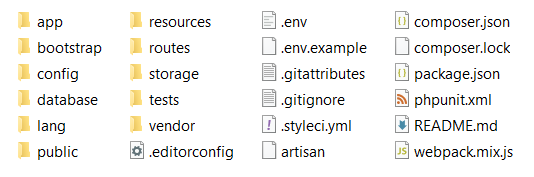
\includegraphics[width=0.9\textwidth]{img/laravel_struktura.png} %% vložení samotného obrátku
			\caption{Obecná struktura nově vygenerovaného Laravel projektu} %% popisek obrázku, nezapomeň na citace!
			\label{fig:laravel_str} %% označení až budeš chtít na obrázek odkazovat
		\end{figure}
	%% obrázek struktury složky
	Jak můžeme na obrázku \ref{fig:laravel_str} vidět, celý projekt je složen z mnoha složek a souborů. Jelikož podrobný rozbor jednotlivých částí není předmětem této práce, tak jsou nejdůležitější části pro implementaci projektu popsány níže jen obecně.
	\begin{itemize}
		\item Složka \textit{app} obsahuje většinu tříd jádra aplikace (obsahuje např. modely či kontrolery) \cite{LaravelDir}
		\item Složka \textit{bootstrap} obsahuje soubory pro zavedení a spuštění aplikace \cite{LaravelDir}
		\item Složka \textit{config} obsahuje konfigurace jednotlivých částí aplikace \cite{LaravelDir}
		\item Složka \textit{database} obsahuje soubory spojené s prací s databázi \cite{LaravelDir}
		\item Složka \textit{lang} obsahuje soubory jazyků a překladů (zde nevyužita) \cite{LaravelDir}
		\item Složka \textit{public} obsahuje soubory, které jsou veřejně dostupné při uživatelské interakci s aplikací (např. při načtení webu v prohlížeči) \cite{LaravelDir}
		\item Složka \textit{resources} obsahuje pohledy a nezkompilované soubory pro celý frontend \cite{LaravelDir}
		\item Složka \textit{routes} obsahuje všechny definice cest aplikace (např. cestu \textit{/api/forms/create} pro vyřízení požadavku vytvoření nového formuláře) \cite{LaravelDir}
		\item Složka \textit{storage} obsahuje primárně záznamy o chodu aplikace a jiné aplikací vygenerované soubory \cite{LaravelDir}
		\item Složka \textit{tests} obsahuje automatizované testy aplikace (zde nevyužita) \cite{LaravelDir}
		\item Složka \textit{vendor} obsahuje závislosti a soubory přídavných balíčků spravované Composerem (viz sekce \ref{sec:composer}), které aplikace používá \cite{LaravelDir} 
		\item Soubor .env držící veškeré důležité administrativní hodnoty jako např. přihlašovací údaje k databázi
		\item Soubor artisan obsahující důležité příkazy pro stavbu aplikace \cite{LaravelArtisan} 
		\item Soubor composer.json držící informace o přídavných balíčcích Composeru (viz sekce \ref{sec:composer}) pro Laravel projekt \cite{ComposerpJSON}
		\item Soubor package.json držící informace o přídavných balíčcích spravovaných pomocí NPM (viz sekce \ref{sec:npm}) pro frontendovou část projektu \cite{NPMpJSON}
		\item Soubor webpack.mix.js obsahující informace pro kompilaci souborů pro frontend \cite{LaravelJSCSS}
	\end{itemize}

	\subsection{Cesty}\label{sec:routes} %%Routes
	Cesty (volně přeložen původní název Routes) jsou využívány abstraktně k rozdělení aplikace - to je myšleno tak, že na každé cestě lze provádět jen úkon, který jí je přiřazen. Tyto cesty mají tvar URL adresy - skládají se z názvu výchozí domény, který je rozšířen o příslušnou cestu (ve formě textového řetězce děleného lomítky), a jsou využívány např. v prohlížeči pro přístup na specifickou stránku. Příkladem může být cesta vytvoření formuláře s příkladovou výchozí doménou \textit{localhost} s portem 8000 \textit{\uv{localhost:8000/forms/create}}. Po zadání této cesty do webového prohlížeče se za splnění podmínek jako spuštění lokálního serveru s aplikací a přihlášení do uživatelského účtu zobrazí požadovaná stránka.
	
	Běžně se v Laravelu tyto cesty definují v souboru \textit{web.php} - v tomto projektu tomu tak ale úplně není, jelikož cesty, kam se uživatel může v aplikaci dostat, jsou definovány ve frontendové části - to také vyplývá z předem dané koncepce aplikace - Laravel má sloužit jen jako API, proto neřeší, jaká data budou v prohlížeči vykreslena - k tomu slouží frontendová část ve VueJS. K těmto účelům je ve zmíněném souboru deklarováno, že na jakékoli cestě se má vrátit prázdný pohled \textit{app} (popsán v části Pohledy), který je pak doplněn o příslušný obsah, který zajišťuje oddělený frontend (viz obrázek \ref{fig:routes_web}). Jedinou výjimkou jsou zde cesty pro resetování hesla předdefinované pro samotný Laravel.
	
	\begin{figure}[H]
		\centering %% příkaz, který ti obrázek zarovná na střed
		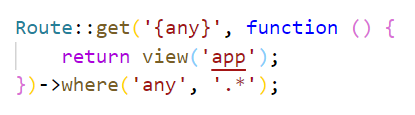
\includegraphics[width=0.6\textwidth]{img/routes/web_routes.png} %% vložení samotného obrátku
		\caption{Část kódu \textit{web.php} vracející pohled \textit{app} na všech cestách} %% popisek obrázku, nezapomeň na citace!
		\label{fig:routes_web} %% označení až budeš chtít na obrázek odkazovat
	\end{figure}
	
	Cesty, které Laravel specificky obsluhuje, jsou v souboru \textit{api.php} (viz. obrázek \ref{fig:routes_api}). Na tyto cesty uživatel v adresním řádku webového prohlížeče vůbec nepřistupuje - jsou využívány ve frontendové části na pozadí. Až zde je vlastně definováno abstraktní rozdělení aplikace - dle cesty se vykonává určitý úkon. 
	
	Tyto API cesty jsou oproti běžným cestám aplikace rozlišeny tak, že mezi výchozí doménu a cestu k dané službě je vložen řetězec \textit{\uv{/api/}} - to je výchozí chování cest v souboru \textit{api.php}. K tomu, aby tyto cesty fungovaly s dalšími službami, bylo nutné je specifikovat v konfiguračních souborech \textit{sanctum.php} a \textit{cors.php}.
	
	\begin{figure}[H]
		\centering %% příkaz, který ti obrázek zarovná na střed
		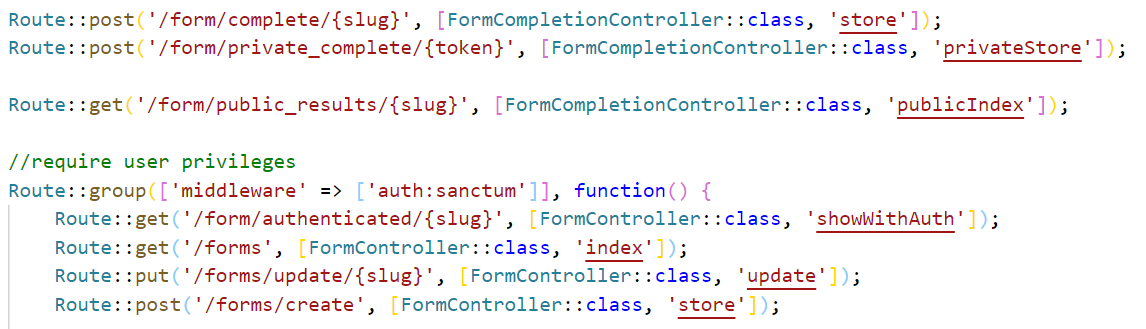
\includegraphics[width=0.9\textwidth]{img/routes/api_routes.png} %% vložení samotného obrátku
		\caption{Část kódu \textit{api.php}} %% popisek obrázku, nezapomeň na citace!
		\label{fig:routes_api} %% označení až budeš chtít na obrázek odkazovat
	\end{figure}
	
	Zmíněné cesty jsou rozděleny do dvou skupin - s veřejným přístupem (bez přihlášení) nebo s privátním přístupem (s přihlášením). Veřejné cesty jsou obslouženy vždy, privátní cesty jsou obslouženy jen pokud jsou společně s příslušnými daty odeslány údaje o přihlášení (tj. autorizační tokeny) - ty si autonomně spravuje balíček Laravel Sanctum pro zabezpečení single-page aplikací. Ke každé cestě je přidělen úkon, který je deklarován v příslušném kontroléru. 
	
	Zmíněné cesty mají také deklarováno, jakou metodu komunikace používají. V této implementaci byly využity zejména tyto metody: standardní GET a POST, ale také PUT pro aktualizaci dat nebo DELETE pro mazání dat.
	
	V rámci popisu aplikace jsou zde tabulky s jednotlivými cestami a jejich úkony - tabulka \ref{tab:verejne_cesty} obsahuje veřejné cesty, tabulka \ref{tab:cesty_s_prihlasenim} obsahuje cesty s přihlášením. Hodnoty u cest ve složených závorkách značí určitou proměnnou přenášenou přes URL adresu (např. \textit{slug} jako identifikátor formuláře).
	
	\newpage
	\begin{table}[H]
		\centering
		\begin{tabular}{ | p{0.4\linewidth} | p{0.1\linewidth} | p{0.4\linewidth} | } 
			\hline
			\textbf{Cesta (\texttt{/api/} + řetězec níže)} & \textbf{Metoda} & \textbf{Funkce} \\ 
			\hline
			\texttt{/login} & POST & Přihlášení uživatele \\ 
			\hline
			\texttt{/register} & POST & Registrace uživatele \\ 
			\hline
			\texttt{/logged\_user} & GET & Vrácení přihlášeného uživatele \\ 
			\hline
			\texttt{/forgot\_password} & POST & Zaslání emailu pro resetování hesla \\
			\hline
			\texttt{/reset\_password} & POST & Resetování hesla \\
			\hline
			\texttt{/form/\{slug\}} & GET & Vrácení veřejného formuláře \\
			\hline
			\texttt{/private\_form/\{token\}} & GET & Vrácení privátního formuláře \\
			\hline
			\texttt{/form/complete/\{slug\}} & POST & Odeslání odpovědi na veřejný formulář \\
			\hline
			\texttt{/form/private\_complete/\{token\}} & POST & Odeslání odpovědi na privátní formulář \\
			\hline
			\texttt{/form/public\_results/\{slug\}} & GET & Vrácení veřejných výsledků formuláře \\
			\hline
		\end{tabular}
		\caption{Veřejné cesty}
		\label{tab:verejne_cesty}
	\end{table}

	\begin{table}[H]
		\centering
		\begin{tabular}{ | p{0.4\linewidth} | p{0.1\linewidth} | p{0.4\linewidth} | } 
			\hline
			\textbf{Cesta (\texttt{/api/} + řetězec níže)} & \textbf{Metoda} & \textbf{Funkce} \\ 
			\hline
			\texttt{/form/authenticated/\{slug\}} & GET & Vrácení formuláře pro administrátorský přístup \\
			\hline
			\texttt{/forms} & GET & Vrácení formulářů, které patří uživateli \\
			\hline
			\texttt{/forms/update/\{slug\}} & PUT & Aktualizace formuláře \\
			\hline
			\texttt{/forms/create} & POST & Vytvoření formuláře \\
			\hline
			\texttt{/forms/\{slug\}} & DELETE & Odstranění formuláře \\
			\hline
			\texttt{/form/duplicate} & POST & Duplikování formuláře \\
			\hline
			\texttt{/form/results/\{slug\}} & GET & Vrácení výsledků formuláře \\
			\hline
			\texttt{/form/results/\{slug\}/download} & GET & Export výsledků formuláře ke stažení \\
			\hline
			\texttt{/form/results/\{slug\}/\newline publish\_results} & POST & Nastavení veřejných výsledků \\
			\hline
			\texttt{/forms/update\_access/\{slug\}} & PUT & Úprava přístupu k formuláři \\
			\hline
			\texttt{/logout} & POST & Odhlášení uživatele \\
			\hline
			\texttt{/change\_password} & PUT & Změna hesla \\
			\hline
			\texttt{/delete\_account} & POST & Smazání účtu uživatele \\
			\hline
		\end{tabular}
		\caption{Cesty s přihlášením}
		\label{tab:cesty_s_prihlasenim}
	\end{table}
	\newpage
	
	\subsection{Modely}
	Modely slouží k mapování jednotlivých dat z databáze a jsou zprostředkovány pomocí objektově-relačního mapovacího balíčku Eloquent. Pro správnou funkčnost musí být zajištěno, že má každá tabulka v databázi vlastní model. Díky tomuto přístupu lze s daty manipulovat tak, že vytvoříme instanci příslušné třídy a na ní voláme příslušné metody (např. \textit{update} pro změnu záznamů) - nemusíme tedy vytvářet jednotlivé SQL příkazy pro všechny požadované úkony \cite{LaravelORM}.
	
	V rámci tohoto projektu vzniklo mnoho modelů, které mapují většinu tabulek databáze (v kontextu mnou vytvořených modelů nejsou vytvořeny modely např. pro předgenerované tabulky jako \textit{migrations} nebo \textit{failed\_jobs}). Kromě samotné funkce mapování dat z databáze jim můžeme přiřazovat různé vlastnosti a metody, díky kterým lze měnit např. chování při předávání dat. Nejdůležitější a v projektu použité jsou v následujícím seznamu:
	
	\begin{itemize}
		\item Metody vytvářející vazby mezi modely - Ty určují jednotlivé vztahy mezi modely a slouží k jednodušší práci s daty. Existuje mnoho metod - např. belongsTo (označuje, komu samotný model náleží) či hasOne/hasMany (označuje, které model/y samotnému modelu patří). \cite{LaravelORM}
		\item Vlastnost \textit{fillable} - Ta určuje, do kterých atributů může být na vrstvě webové aplikace zapisováno. Nenapíšeme sem tedy např. \textit{id}, které většinou chceme doplnit až při uložení do databáze samotnou databází. \cite{LaravelORM}
		\item Vlastnost \textit{visible} - Ta určuje, které atributy jsou ve vrácených datech z databáze viditelné a tedy poslané dále (myšleno na frontend aplikace). Např. z bezpečnostního hlediska sem nenapíšeme atribut uživatelského hesla, který by neměl být obecně předáván mimo server. \cite{LaravelORM}
		\item Vlastnost \textit{table} - Ta slouží k přesnému určení tabulky pomocí jejího jména, ke které se vytvořený model vztahuje. \cite{LaravelORM}
		\item Vlastnost \textit{with} - Ta slouží k výchozímu připojení dalších dat z jiného modelu ke stávajícímu setu dat modelu. K takovému úkonu je nutné mít vytvořené vazby pomocí příslušných metod. \cite{LaravelORM}
	\end{itemize}

	Každý model většinou nevyužívá všechny zmíněné činnosti, ale jen ty, které jsou pro jeho typ důležité. Příkladem je zde uveden poměrně rozsáhlý model formuláře \textit{Form}. Podobným způsobem jsou vytvořeny i ostatní modely.
	
	Třída modelu Form reprezentuje jednotlivé formuláře. Odkazuje se na stejnojmennou tabulku \textit{forms}, ze které přebírá data. Má definované vlastnosti (viz obrázek \ref{fig:model_vlastnosti}): \textit{fillable} (např. jméno formuláře, popis formuláře, čas spuštění, ID uživatele, kterému formulář patří,...), \textit{visible} (např. atributy jako jméno formuláře, odkaz na formulář či popis formuláře, ale také názvy atributů, které jsou přidávány v průběhu práce s daty, a názvy metod vytvářejících vazby mezi některými dalšími modely (viz obrázek \ref{fig:model_metody}) jako např. pro model uživatele, pro kterého platí, že mu formulář musí náležet) a \textit{with} (zde jen název vazbové metody pro model elementu formuláře, u kterého platí, že musí formuláři náležet a že jednomu formuláři může náležet i více elementů). Samotná definice provázání modelu s tabulkou v databázi pomocí vlastnosti table zde není potřeba - Laravel umí u jednoduše pojmenovaných modelů vygenerovaných pomocí Artisan skriptů tuto vlastnost vnitřně doplnit.
	
	%%obrázek modelu php
	%%\newpage
	\begin{figure}[H]
		\centering
		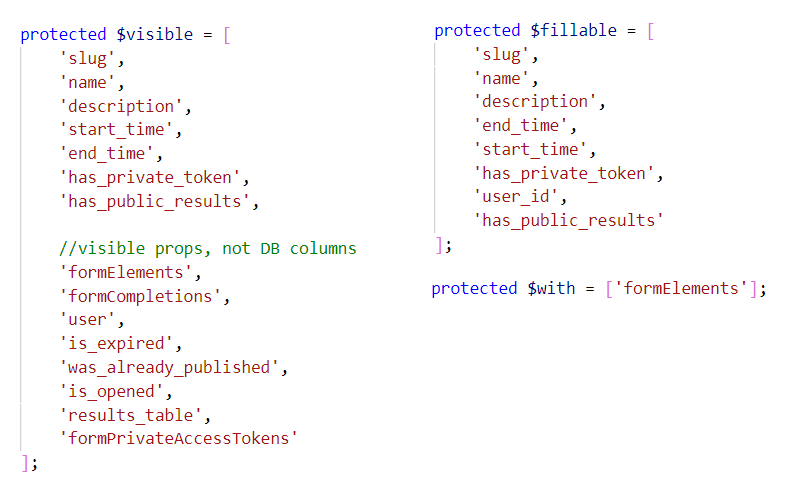
\includegraphics[width=0.85\textwidth]{img/form_model/vlastnosti.png}
		\caption{Zmíněné vlastnosti modelu formuláře}
		\label{fig:model_vlastnosti}
	\end{figure}
	
	\begin{figure}[H]
		\centering
		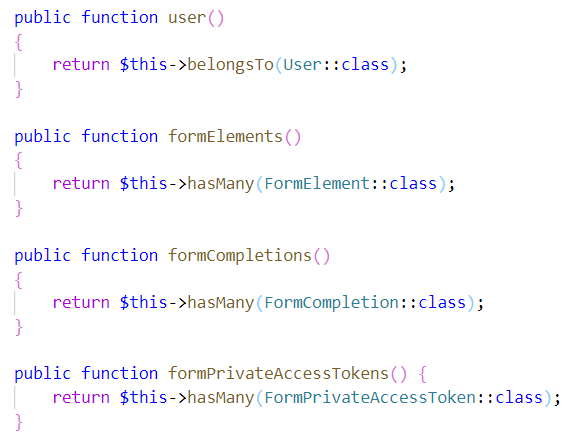
\includegraphics[width=0.7\textwidth]{img/form_model/metody.png}
		\caption{Zmíněné metody modelu formuláře}
		\label{fig:model_metody}
	\end{figure}
	%%\newpage
	
	\subsection{Kontroléry}
    Kontroléry jsou jednou z nejdůležitějších částí celé aplikace - probíhají v nich všechny požadované činnosti, které voláme přes specifické cesty. Obecně zajišťují veškerou administrativu nad příslušným modelem - tzn. např. model formuláře by měl mít svůj kontrolér. Většinou v nich najdeme metody pro vrácení všech prvků nebo konkrétního prvku příslušného modelu či metody pro ukládání, aktualizaci a mazání jednotlivých prvků.
    
    Kontroléry v této aplikaci (viz obrázek \ref{fig:kontroler}), resp. jejich metody, jsou nastaveny tak, aby v případě chyby vrátily příslušný stavový kód pro jednoznačnou identifikaci chyby. Pokud se chyba nevyskytne, jsou navrácena příslušná data se stavovým kódem 200, který značí úspěch akce. 
    
    \begin{figure}[H]
    	\centering
    	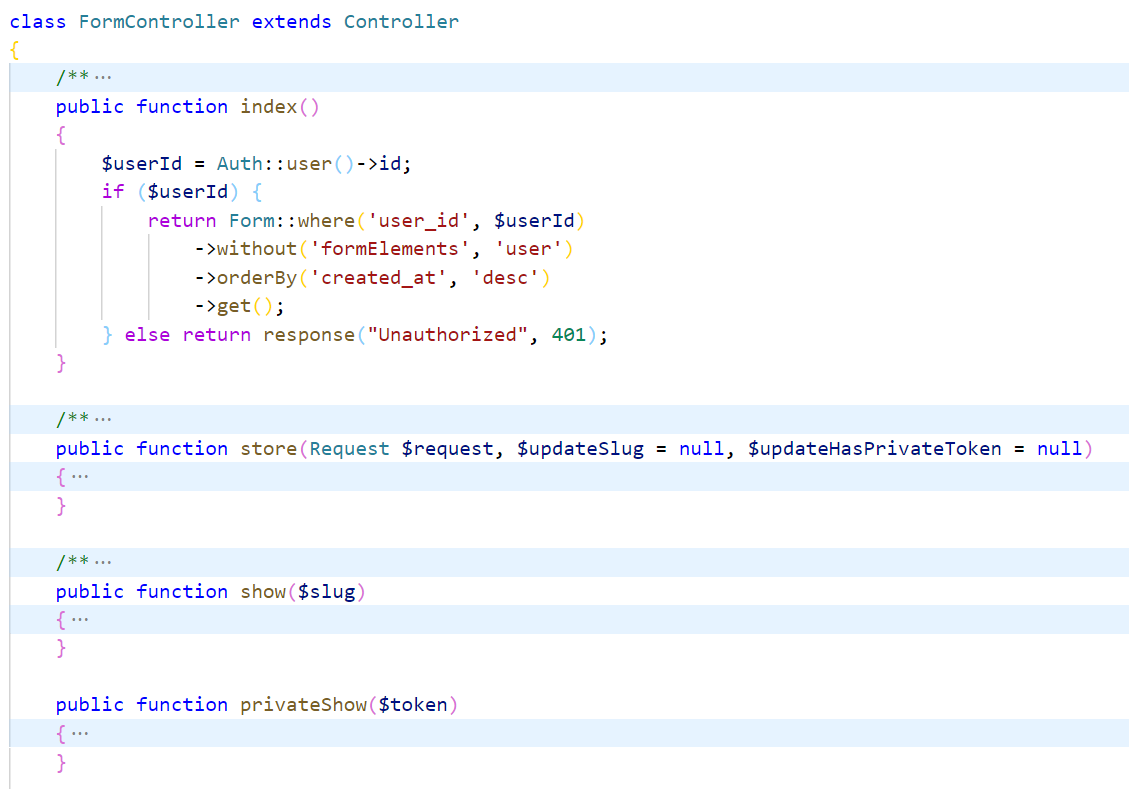
\includegraphics[width=0.85\textwidth]{img/kontroler.png}
    	\caption{Ukázka části kódu kontroléru (Kontrolér formuláře)}
    	\label{fig:kontroler}
    \end{figure}
    
    Konkrétní postupy, jak se jednotlivé činnosti provádí, jsou popsány v jiné sekci práce.
		\subsubsection{Kontrolér formuláře}
		Kontrolér formuláře, jak už z názvu vyplývá, pracuje s daty jednotlivých formulářů. Kromě výše zmíněných běžných metod obsahuje metodu pro vrácení privátního formuláře, metodu pro duplikaci formuláře, metodu pro vrácení formuláře s dodatečnými daty pro majitele formuláře, metodu pro nastavení veřejných výsledků či metodu pro úpravu přístupu k formuláři (nastavení veřejného nebo privátního formuláře).
		
		\subsubsection{Kontrolér vyplnění formuláře}
		Kontrolér vyplnění formuláře je oproti předchozímu kontroléru chudší. V rámci běžných metod neobsahuje např. metodu pro úpravu či smazání odpovědi. Oproti tomu ale disponuje speciální metodou pro export všech odpovědí do stáhnutelného formátu MS Excel, metodou pro uložení odpovědi z privátního formuláře či metodou pro zobrazení veřejných výsledků.
		
		\subsubsection{Kontrolér uživatele}
		Kontrolér uživatele slouží ke správě uživatelů. Obsahuje základní metody pro registraci, přihlášení a odhlášení, ale i pro změnu hesla (i při zapomenutém hesle) či smazání účtu.
	
	\subsection{Exporty}\label{sec:exports}
	Exporty, resp. jejich třídy, slouží k definování vzhledu a způsobu uložení dat v určitém formátu. Exportovat můžeme různá data do různých formátů (např. obrázek do formátu PNG, list nějakých záznamů do tabulky formátu CSV,...).
	
	V rámci tohoto projektu byl export potřeba jen v jednom případě - pro exportování výsledků vyplnění formuláře pro majitele formuláře do formátu MS Excel. K tomuto účelu byl využit přídavný balíček \uv{maatwebsite/excel}, který zajišťuje veškerou administrativu nad věcmi s tímto úkonem spojených. Jakým způsobem jsou data exportována je popsáno v jiné sekci práce.
	
	\subsection{Maily}
	Maily, resp. jejich třídy, slouží k definování vzhledu a obsahu emailu. Poté, co se vytvoří instance této třídy, která je hydratována, data jsou předána příslušnému pohledu, který je poté poslán na příslušné emaily.
	
	Způsoby a principy, kterými jsou emaily rozesílány, zde nejsou popsány - jednak jsou předdefinované Laravelem a zároveň nejsou předmětem této práce. Jediné, co bylo potřeba k zprovoznění emailového klienta, bylo vyplnit příslušné konfigurační údaje (např. protokol pro přenos nebo port na emailový server) a přihlašovací údaje k emailu, ze kterého jsou emaily rozesílány. K těmto účelům byl v implementaci projektu na produkční verzi použit Google Gmail.
	
	\subsection{Migrace databáze}
	Migrace databáze jsou určeny k deklaraci struktury jednotlivých tabulek v databázi. Obecně mají dvě metody: \textit{up} pro vytvoření předdefinované tabulky a \textit{down} pro odstranění tabulky z databáze. Tyto migrace se v Laravelu běžně generují pomocí Artisan skriptů.
	
	V implementaci tohoto projektu se využívala primárně metoda \textit{up}, kde se specifikovaly jednotlivé názvy a typy atributů tabulky. Těmto atributům lze přidávat další různé vlastnosti (v migraci zapsány jako metody) jako např. \textit{nullable} (možnost vložení prázdné hodnoty \textit{null} do atributu), \textit{default} (možnost nastavení výchozí hodnoty atributu při vytvoření) či \textit{unique} (možnost nastavení unikátní hodnoty atributu ve sloupci).
	
	Kromě zmíněných vlastností bylo ještě nutné specifikovat tzv. cizí klíče, které slouží k vytvoření relací mezi ostatními databázovými objekty a k celkovému provázání dat. Jedná se o samostatné atributy, které většinou obsahují ID jiného objektu v databázi - tím je zaručeno, který řádek v tabulce patří k řádku/řádkům jiné tabulky. 
	
	 \begin{figure}[h]
		\centering
		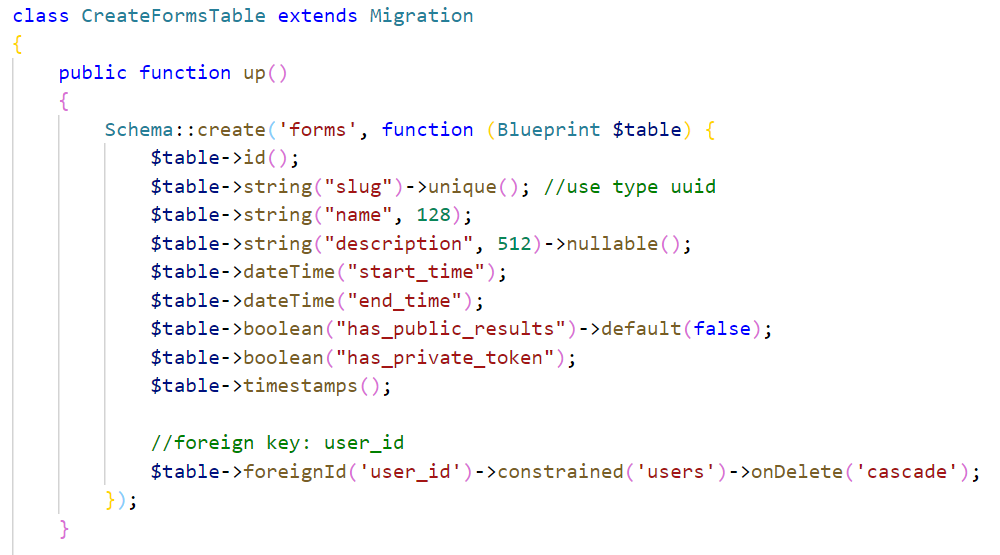
\includegraphics[width=0.85\textwidth]{img/migrace.png}
		\caption{Ukázka části kódu migrace (Tabulka pro formuláře)}
		\label{fig:migrace}
	\end{figure}
	
	V Laravel migraci je toto deklarováno pomocí vlastnosti \textit{constrained}, ve které specifikujeme, se kterou tabulkou lze data ze současné tabulky spojovat. Pokud jsou i ostatní tabulky vytvořeny vygenerovanými migracemi, nemusíme ani specifikovat, který sloupec bude z jiné tabulky sloužit k provázání - k tomu Laravel standardně používá sloupec \textit{id}.
	
	Poslední věcí, která byla nutná k zachování referenční integrity dat v databázi pro implementaci projektu, bylo u několika tabulek specifikovat chování při smazání řádku z tabulky, který je provázán s jinou tabulkou. K tomu slouží vlastnost \textit{onDelete}, kde toto chování deklarujeme. V tomto projektu je použit způsob chování \uv{kaskáda}. Ta funguje v případě mazání tak, že pokud je smazán rodičovský (nadřazený) objekt, tak jsou smazány všichni potomci (podřazené objekty) \cite{CascadeDel}.
		
		\subsubsection{Testovací data}
		K tomu, aby bylo možné aplikaci rozumně testovat, je nutné mít v databázi nějaká data. Pokud bychom vždy ručně tato data přidávali, trvalo by to enormní množství času - k~těmto účelům v Laravelu existují tzv. Factories a Seeders.
		
		Factories (volně přeloženo jako Továrny) slouží k vygenerování výplňových dat, která jsou použita primárně při vývoji aplikace. Tyto továrny na vymyšlená data jsou poté použita v Seederu (volně přeloženo jako Rozsévač), který provádí všechny úkony jako vymazání všech současných dat databáze a následné naplnění daty z továren.
	
	\subsection{Pohledy}
	Pohledy jsou šablony ve formátu PHP (spravované balíčkem \uv{Blade}), pomocí kterých Laravel nativně vykresluje data uživateli. Poté, co jsou takové šabloně data předána (např. pomocí kontroléru), je šablona následně převedena na HTML formát, který je čitelný např. pro webový prohlížeč. Obvykle také obsahuje závislosti na různé přídavné soubory - např. Javascript nebo CSS soubory. 
	
	V tomto projektu (jak již bylo zmíněno výše) je pro vykreslení ve webovém prohlížeči použit pouze jeden pohled s názvem \textit{app} (viz obrázek \ref{fig:pohled_app}). Tato šablona kromě standardní HTML hlavičky a běžných referenci na Javascriptové nebo CSS soubory obsahuje pouze tělo obsahující jen jeden oddíl s ID \textit{app}. Na tento oddíl díky referenci na ID poté oddělený frontend ve VueJS připojuje další jednotlivé elementy stránky - tyto elementy a další postupy jsou dále popsány ve frontendové části práce.
	
	\begin{figure}[h]
		\centering
		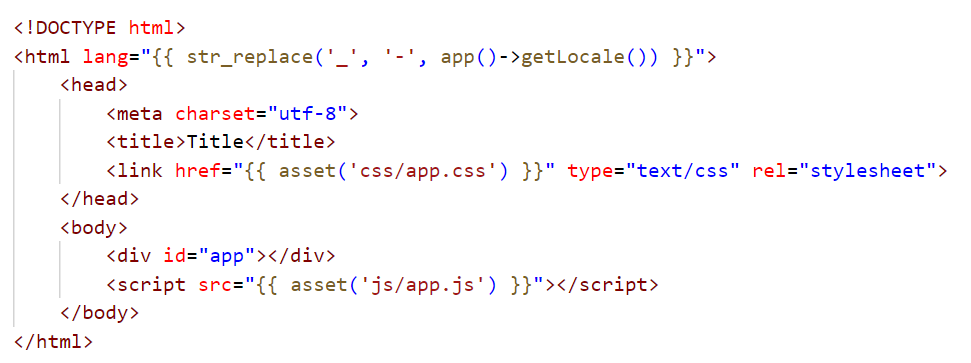
\includegraphics[width=0.9\textwidth]{img/pohled_app.png}
		\caption{Šablona pohledu \textit{app} (pro účely této práce upravena)}
		\label{fig:pohled_app}
	\end{figure}
	
	\subsection{Průběh jednotlivých činností}
	V této části jsou popsány postupy, jak se jednotlivé akce zpracovávají na serveru a jak jsou data předávána databázi či uživateli webové stránky. Úkony jsou rozděleny tak, jak jsou zapsány v kontrolérech. Z hlediska kódu je každý úkon metodou kontroléru.
	
	Každá z těchto metod vrací po provedení úkonu většinou předdefinovaný stavový kód označující, zda se činnost provedla úspěšně či nikoliv. Zde (tabulka \ref{tab:http_stavove_kody}) je seznam přímo využitých stavových kódů, které jsou serverem předávány.
	
	\begin{table}[H]
		\centering
		\begin{tabular}{ | p{0.1\linewidth} | p{0.3\linewidth} |  p{0.5\linewidth} |} 
			\hline
			\textbf{Stavový kód} & \textbf{Hláška} & \textbf{Popis hlášky} \\ 
			\hline
			200 & OK & Operace proběhla úspěšně. \\
			\hline
			204 & No Content & Operace proběhla úspěšně, ale žádná data nebyla klientovi poslána. \\
			\hline
			400 & Bad Request & Server nerozumí požadavku. \\
			\hline
			401 & Unauthorized & Server vyžaduje autorizaci. \\
			\hline
			404 & Not Found & Požadovaná stránka nebyla nalezena. \\
			\hline
			410 & Gone & Požadovaná stránka již není dostupná. \\
			\hline
			423 & Locked & Požadovaný zdroj je uzamčen. \\
			\hline
			500 & Internal Server Error & Obecná chybová hláška serveru - došlo k neočekávané chybě. \\
			\hline
		\end{tabular}
		\caption{Využité stavové kódy HTTP \cite{HTTPKody1} \cite{HTTPKody2}}
		\label{tab:http_stavove_kody}
	\end{table}

	Nutno zmínit, že stavový kód \uv{200 (OK)} je v této implementaci projektu automaticky odesílán v případě, že v průběhu vyřizování požadavku není zaznamenána žádná chyba. Dále v práci proto nebude jeho odesílání zmiňováno.
	
		\subsubsection{Manipulace s formuláři}
		Tato část popisuje veškerou administrativu nad formuláři.
		
			\subsubsubsection{Vytvoření formuláře}\label{sec:form_store}
			Metoda s názvem \textit{store} slouží k vytvoření a uložení formuláře s jeho elementy do databáze. Kromě samotného vytvoření se stará o integritu formátu jednotlivých otázek a validitu příslušných atributů formuláře. Při chybě validace předaných dat (pokud není chyba cíleně ignorována) je nejčastěji vrácen stavový kód 400.
			
			Prvním krokem, co funkce provádí, je ověření, zda je uživatel přihlášen (pokud není, je vrácen stavový kód 401). Poté se provádí rozsáhlá validace, která sestává z kontroly základních informací o formuláři (např. název formuláře či data zveřejněni a ukončení zveřejnění), samotných elementů formuláře a dalších parametrů validního formuláře. Před těmito úkony je zkontrolováno, zda požadavek od uživatele vůbec obsahuje nějaká data.
			
			Validace základních informací kontroluje název a popisek formuláře (zda obsahují validní řetězec, u názvu samotné vyplnění - jedná se o povinný atribut), data zveřejnění a ukončení zveřejnění formuláře (zda mají hodnoty správný formát, zda datum ukončení zveřejnění je dále v čase než datum zveřejnění a zda se netvoří už expirovaný formulář s časem ukončení zveřejnění dříve v čase než je aktuální serverový čas), hodnotu vyjadřující přístupnost formuláře (zda bude veřejný nebo privátní) a zda požadavek vůbec obsahuje kolekci otázek. U privátního formuláře jsou také validovány emaily, na které se rozešle pozvánka (tzn. jejich formát).
			
			Další částí je validace elementů. Ty jsou procházeny cyklem, ve kterém se nejprve zjišťuje, zda je vybraný element elementem otázky nebo nové stránky, a kontroluje se správné pořadí na základě vlastnosti \textit{order}. Pokud se jedná o novou stránku, přeskakuje se validace atributů otázky, a pokud má stránka validní hodnotu pro pořadí, je rovnou přemístěna mezi validní elementy. 
			
			V případě elementu otázky je to komplikovanější. Kromě validace pořadí přichází na řadu kontroly vlastností jako jsou typ samotné otázky (zda se jedná o platný typ podporovaný systémem), samotný textový řetězec vyjadřující otázku (zda se jedná o text), atribut vyjadřující, zda se jedná o otázku povinnou, či nikoliv (kontrola typu). Poté, na základě typu, jsou validovány atributy související s typem otázky. Atributy, které jednotlivé typy otázek mají, jsou rozebrány v sekci \ref{sec:form_inputs_types} - u některých ze samotné podstaty vyplývá, co a jak se u nich bude validovat. 
			
			Obecně platí, že u rozsahů délky (tzn. minimální a maximální hodnoty) musí platit, že minimální hodnota je menší než maximální (a to nezávisle na typu - tzn. platí např. i pro datum - i přesto, že jsou data vkládána jako textový řetězec, musí být příslušně převedena a zvalidována). Striktní délka musí být větší než nula. U atributů, kde má být zadána hodnota \textit{true} nebo \textit{false}, kontrolovat validní hodnotu popř. předanou hodnotu převést na validní tvar. Obvykle, pokud se nejedná o povinnou hodnotu, se chyby ignorují - proces pokračuje dále, žádné hodnoty nejsou do těchto atributů uloženy.
			
			Nejkomplikovanější validace probíhá u typu vstupu pro odpověď z výběru předepsaných možných odpovědí. Zde musí být validovány i jednotlivé možnosti odpovědi pro otázku - u nich se kontroluje počet (možností musí jich být více než dvě), zda se jedná o škálu (na základě \textit{true}/\textit{false} hodnoty \textit{has\_hidden\_label} - pokud je tato hodnota \textit{true}, očekává se u všech možností číselný popisek, který je pro danou kolekci možností unikátní), vnitřní pořadí (zda se jedná o čísla tvořící posloupnost 0,1,2,3,...) a samotný text vyjadřující odpověď na otázku (zda se jedná o platnou textovou hodnotu). V případě selhání validace těchto částí chyby nejsou ignorovány a je vrácen příslušný chybový stavový kód. Po této validaci už následuje jen validace rozsahu počtu odpovědí či striktního počtu odpovědí (pokud se jedná o tzv. multiple-choice otázku) - u těchto hodnot platí kromě dříve popsaných pravidel, že musí být v symbióze s počtem možností odpovědí - tzn. zadané hodnoty musí být menší než celkový počet možností.
			
			Po validaci zmíněných přichází na řadu kontrola dalších parametrů. Tím je validace pořadí (elementy musí mít v atributu pořadí číslo, které s ostatními tvoří posloupnost 0,1,2,3,...) a kontrola, zda v kolekci otázek existuje alespoň jedna otázka povinná. Dále je zavedena kontrola umístění elementů nové stránky - pro ty platí, že nesmí stát na začátku a na konci kolekce elementů a že v kolekci nesmí stát dva a více vedle sebe. V případě výskytu chyby je vrácen příslušný chybový stavový kód.
			
			Pokud jsou všechna data validní, tak se začne vykonávat kód pro předejití poškození integrity dat v databázové transakci, kde je v případě tvoření formuláře nejprve vygenerován unikátní identifikátor pomocí balíčku \uv{ramsey/uuid} ve tvaru UUID4. Poté se postupně vytváří příslušné objekty pro jednotlivé prvky formuláře, kterým se předávají zvalidovaná data. Po tomto úkonu se v případě privátního formuláře rozešlou pozvánky na příslušné emaily.
			
			\subsubsubsection{Úprava formuláře}
			Metoda s názvem \textit{update} slouží k editaci formuláře, který zatím nebyl zveřejněn. Díky této metodě lze kromě základních informací měnit i samotné otázky. Co v této metodě ale nelze provést je úprava přístupnosti formuláře a případné přidání emailů k rozeslání pozvánky (k tomu slouží metoda v sekci \ref{sec:form_accessibility}).
			
			Při volání metody se nejprve ověří, zda je uživatel přihlášen (pokud není, je vrácen stavový kód 401) a zda požadovaný formulář existuje (pokud ne, je vrácen stavový kód 404). Poté přichází na řadu kontrola časů - kontroluje se, zda už nebyl formulář zveřejněn na základě data zveřejnění formuláře (atribut musí být dále v čase než je serverový čas). Pokud tato podmínka není splněna, je vrácen stavový kód 400.
			
			Dále je spuštěna databázová transakce, ve které se nejprve vygeneruje dočasný identifikátor \textit{slug} formuláře ve tvaru UUID4. Poté se všechna data z požadavku uživatele předají metodě \textit{store} (popsána v sekci \ref{sec:form_store}), která přidá do databáze formulář s předanými úpravami. Kromě dat z požadavku se metodě poskytnou i další data: dočasný identifikátor, který slouží k identifikaci přidaného upraveného formuláře a informace o tom, zda byl upravovaný formulář veřejný nebo privátní. Dočasný identifikátor je použit místo vygenerovaného identifikátoru použitého přímo v metodě \textit{store}. Předávaná informace o přístupnosti slouží k tomu, aby upravený formulář tuto vlastnost neztratil a aby nebyly znovu rozeslány pozvánky na příslušné emaily, což je nativní chování metody \textit{store}. 
			
			Poté, pokud nebyl uživatelský požadavek validní dle metody pro přidání formuláře, je vrácen příslušný stavový kód pocházející přímo ze zmíněné metody. Pokud ale vše v metodě \textit{store} proběhlo bez problému, následují další činnosti. Pokud se jedná o veřejný formulář, původní (neupravený) formulář (a s ním i další objekty na něj navázané) je smazán pomocí metody \textit{destroy} (popsána v sekci \ref{sec:form_destroy}) a u upraveného formuláře je přepsán identifikátor na hodnotu identifikátoru, kterou disponoval neupravený formulář. V případě, že je upravený formulář privátní, se prvně do dočasné proměnné uloží všechny přístupové tokeny. Poté se původní formulář smaže a nahradí se identifikátor stejně jako u veřejného formuláře. Nakonec se vytvoří kopie tokenů na základě dat v dočasné proměnné zmíněné dříve, které se liší jen v hodnotě ID formuláře (to, jelikož byl de facto vytvořen nový formulář, musí odkazovat na upravený formulář). Na neočekávané chyby je vrácen stavový kód 500.
			
			\subsubsubsection{Duplikování formuláře}\label{sec:form_dupl}
			Metoda s názvem \textit{duplicateWithAuth} slouží k duplikování formuláře - tzn. lze vytvořit nový formulář, který obsahuje stejné otázky a vlastnosti (tj. jméno formuláře, datum zveřejnění, datum ukončení zveřejnění,...), jako formulář, u kterého byla požadována duplikace. Zmíněné vlastnosti při tomto procesu lze modifikovat, otázky ne.
			
			Metoda funguje tak, že prvně ověří, zda je uživatel přihlášen (pokud ne, vrátí stavový kód 401), poté zkontroluje zda požadovaný formulář existuje a zda patří přihlášenému uživateli. Dále jsou validovány všechny předané hodnoty vlastností formuláře, které již byly zmíněné - tzn. zda vůbec v požadavku na duplikaci existují a zda jsou správného typu (v případě jakékoliv očekávané chyby je vrácen kód 400). 
			
			U hodnot pro čas zveřejnění a ukončení zveřejnění se validuje příslušný formát data, zda není čas zveřejnění větší (déle v čase) než čas ukončení zveřejnění či zda není vytvářen už expirovaný formulář (tzn. aktuální serverový čas je déle v čase než čas ukončení zveřejnění). 
			
			Poté probíhá kontrola nastavení přístupnosti formuláře - při duplikaci lze změnit tento atribut. Pokud je tento atribut nastaven jako \textit{true} (tzn. formulář je privátní, lze k němu přistupovat jen s tokenem), kontrolují se předané emaily (zda mají validní tvar), na které se bude rozesílat pozvánka.
			
			Nakonec se vygeneruje nový identifikátor ve tvaru UUID4 a metoda se pokouší příslušná data uložit do databáze. Zde vzniká nový objekt formuláře, kterému jsou předány příslušné vlastnosti (tj. ID uživatele, vygenerovaný identifikátor, data z požadavku duplikace). S tím podobně vznikají i příslušné objekty pro uložení jednotlivých elementů formuláře (tj. otázky nebo nové stránky), jejichž vlastnosti jsou přebírány a kopírovány z duplikovaného formuláře. Nakonec, pokud je formulář nastaven jako privátní, jsou rozeslány pozvánky na zvalidované emaily. Tento proces probíhá v databázové transakci.
			
			Při úspěchu je vrácena odpověď s identifikátorem nově vzniklého formuláře (duplikátu). Ten je určen pro frontendovou část projektu k přesměrování.
								
			\subsubsubsection{Úprava přístupnosti formuláře}\label{sec:form_accessibility}
			Metoda s názvem \textit{updateAccess} slouží k úpravě přístupnosti formuláře. V ní lze nastavit, zda je formulář veřejný, nebo privátní (s tím je možné nastavit, na které emaily lze dodatečně poslat pozvánku či kterým emailům s pozvánkou odebrat přístup ve formě invalidace tokenu).
			
			V rámci zpracování dat je nejprve kontrolováno, zda požadavek obsahuje vůbec nějaká data (pokud ne, je vrácen stavový kód 400). Poté se kontroluje přihlášení uživatele (pokud není přihlášen, je vrácen stavový kód 401) a zda požadovaný formulář s příslušným vlastníkem existuje (pokud ne, je vrácen stavový kód 404). Další akce jsou prováděny jen pokud existuje v požadavku uživatele atribut \textit{has\_private\_token} s platnou hodnotou (pokud neexistuje, je vrácen stavový kód 400). Po těchto kontrolách se dále celý proces dělí na dvě logické větve. 
			
			První větev je podmíněna tím, že se zmíněný předaný atribut \textit{has\_private\_token} se rovná \textit{true} (tzn. formulář bude privátní). V takovém případě se nejprve zvalidují předané emaily, na které má být odeslána nová pozvánka (pokud dojde k chybě ve validaci samotných emailů, je vrácen kód 400). Poté, pokud byl měněný formulář veřejný (tzn. před tímto úkonem se jeho hodnota \textit{has\_private\_token} rovnala \textit{false}), se formuláři v databázi přepisuje zmíněný atribut \textit{has\_private\_token} na \textit{true} a vytváří se nové tokeny pro předané emaily, na které je poté rozeslána pozvánka. Pokud byl ale měněný formulář už privátní, tak jsou, společně s vytvořením nových tokenů a rozesláním pozvánek, zneplatněny pozvánky, které byly zaslané na majitelem předané emaily - tzn. po validaci těchto dat jsou z databáze vymazány tokeny, ke kterým jsou vázány příslušné emaily z uživatelského požadavku. Uživatelům, kterým byla pozvánka zneplatněna, se žádný oznamovací email nezasílá.
			
			Druhá větev je podmíněna tím, že zmíněný předaný atribut \textit{has\_private\_token} se rovná \textit{false} a atribut požadovaného formuláře \textit{has\_private\_token} se rovná \textit{false} (tzn. formulář bude převeden na veřejný). V takovém případě proběhne triviální smazání všech privátních tokenů, které se na příslušný formulář váží. Žádný oznamovací email se uživatelům s pozvánkou neposílá.
			
			Veškeré databázové operace spojené se zmíněnými úkony probíhají pro zachování integrity dat v transakcích.
			
			\subsubsubsection{Zveřejnění výsledků formuláře}\label{sec:form_publish_results}
			Metoda s názvem \textit{publishResults} slouží k modifikaci přístupu k výsledkům formuláře pro běžnou veřejnost. Zde lze nastavit, zda jsou výsledky veřejné či nikoliv. Pokud jsou výsledky zveřejněny, lze zvolit, které otázky jsou skryté a které jsou zveřejněné.
			
			Funkce nejprve zkontroluje, zda požadavek obsahuje vůbec nějaká data (pokud ne, je vrácen stavový kód 400). Poté kontroluje přihlášení uživatele (pokud není přihlášen, je vrácen stavový kód 401) a zda požadovaný formulář s příslušným vlastníkem existuje (pokud ne, je vrácen stavový kód 404). Po těchto kontrolách jsou validována předaná data v požadavku na server.
			
			V rámci zmíněných dat se nejprve validuje předaný atribut \textit{has\_public\_results}, který stanovuje, zda má formulář veřejné výsledky - tzn. zda má platnou hodnotu. Poté, pokud je předchozí hodnota \textit{true} (tzn. výsledky budou zveřejněny), jsou procházena a validována všechna data z uživatelova požadavku, která představují jednotlivé otázky a jejich atribut zveřejnění. Zde se kontroluje, zda otázky vůbec náleží požadovanému formuláři (pomocí \textit{id}) - pokud ano, jsou dále předávány společně s informací, zda mají být tyto otázky veřejné, nebo ne (neplatná data v této části jsou ignorována). Zároveň musí platit, že v případě zveřejnění výsledků formuláře musí být alespoň jedna otázka veřejná (pokud toto neplatí, je vrácen stavový kód 400).
			
			Poté se metoda pokouší tato data uložit do databáze. Nejprve přepisuje atribut formuláře \textit{has\_public\_results}, poté, na základě tohoto atributu, manipuluje s jednotlivými elementy. Pokud je zmíněný atribut \textit{true}, tak jsou jednotlivé elementy modifikovány podle zvalidovaných dat (tzn. pokud mají být veřejné, je jim nastaven stejnojmenný atribut \textit{has\_public\_results} na true, v opačném případě na \textit{false}). Pokud je ale zmíněný atribut formuláře \textit{false}, je všem elementům zmíněný atribut zveřejnění nastaven na \textit{false} (tzn. všechny odpovědi jsou skryty). Celý proces probíhá v transakci.
			
			\subsubsubsection{Mazání formuláře}\label{sec:form_destroy}
			Metoda s názvem \textit{destroy} slouží k odstranění formuláře a jeho přidružených elementů.
			
			V koncepci je metoda velice jednoduchá - poté, co se zkontroluje, zda je uživatel přihlášen (pokud ne, je vrácen stavový kód 401), zda vůbec formulář s předaným \textit{slug} identifikátorem patřící přihlášenému uživateli v databázi existuje (pokud ne, je vrácen stavový kód 404), je pomocí příslušné nativní metody \textit{delete()} smazán. Tento proces také probíhá v transakci.
			
			\subsubsubsection{Vrácení všech formulářů uživateli}
			Metoda s názvem \textit{index} je určena k vrácení všech formulářů, které patří přihlášenému uživateli. To slouží k hydrataci úvodní stránky uživatele - jedná se o přehled všech vlastněných formulářů. 
			
			Tato funkce nejprve ověří, zda je uživatel přihlášen. Pokud přihlášen je, vrátí uživateli všechny jeho formuláře bez elementů formuláře a bez dat o uživateli, které se obecně k datům připojují. Tento set formulářů je seřazen podle doby vytvoření formuláře sestupně. Pokud přihlášen není, je vrácen stavový kód 401. 
			
			\subsubsubsection{Vrácení informací o formuláři majiteli}
			Metoda s názvem \textit{showWithAuth} má za účel vrátit celý formulář a data s ním spojená pro jeho vlastníka. Tato data poté slouží k hydrataci stránky s přehledem informací o formuláři.
			
			Funkce nejprve zkontroluje, zda je uživatel přihlášen. Pokud není, je navrácen stavový kód 401. V případě, že je uživatel přihlášen, se v databázi vyhledává formulář na základě předaného identifikátoru \textit{slug}. Pokud formulář není nalezen, je vrácen stavový kód 404, a pokud nepatří přihlášenému uživateli, je vrácen kód 401. 
			
			Po zmíněných kontrolách se k objektu formuláře připojují tři atributy: \textit{is\_expired} (rovná se \textit{true}, pokud je serverový čas dále v čase než čas ukončení zveřejnění), \textit{was\_already\_published} (rovná se \textit{true}, pokud je serverový čas dále v čase než čas zveřejnění formuláře) a \textit{is\_opened} (rovná se \textit{true}, když neplatí \textit{is\_expired} a zároveň platí \textit{was\_already\_published} - tzn. když je formulář dostupný k vyplnění). Po připojení těchto vlastností je celý formulář s příslušnými vlastnosti vrácen.
			
			Pokud je formulář nastaven jako privátní, tak jsou k celému objektu formuláře ještě připojeny záznamy o privátních tokenech. Tyto záznamy slouží pro vlastníka formuláře k výpisu emailů, kterým byla poslána pozvánka a které mají v době vykonávání této metody oprávnění k vyplnění formuláře. Připojené záznamy o tokenech samotný token neobsahují (resp. je skrytý pro vlastníka formuláře) - to slouží k tomu, aby nebylo možné dohledat, který token patří ke kterému emailu. Zároveň to znemožňuje jednoduše odpovědět za člověka, kterému byla odeslána pozvánka k vyplnění.
			
			\subsubsubsection{Vrácení konkrétního veřejného formuláře}\label{sec:form_show}
			Metoda s názvem \textit{show} je určena k vrácení konkrétního veřejného formuláře. To slouží k hydrataci stránky určené k vyplnění veřejného formuláře - obsahuje veškeré náležitosti s tímto úkonem spojené.
			
			V rámci celého procesu funkce nejprve ověří, zda v databázi existuje formulář s požadovaným identifikátorem \textit{slug}. Pokud ne, je vrácen stavový kód 404. Pokud ale nalezen je, provádí se několik kontrol - když kontrolami projde, je navrácen formulář s příslušnými elementy.
			
			První se kontroluje, zda zadaný identifikátor neukazuje na privátní formulář - na tento formulář lze přistoupit jen přes token, nikoliv přes zmíněný identifikátor. Pokud se potvrdí přístup přes identifikátor, odešle se jen stavový kód 400.
			
			Dalším faktorem je čas, kdy k formuláři chce uživatel přistoupit. Ověřuje se podle uložených dat o formuláři z databáze, zda je už formulář zveřejněn (pokud není, je vrácen stavový kód 423) nebo zda už formulář neexpiroval (pokud expiroval, je vrácen stavový kód 410). Aktuální čas se bere podle serveru, na kterém je aplikace nasazena.
			
			\subsubsubsection{Vrácení konkrétního privátního formuláře}
			Metoda s názvem \textit{privateShow} funguje podobně jako metoda popsána v sekci \ref{sec:form_show}. Místo identifikátoru \textit{slug} se nejprve vyhledává uživatelem předaný token v databázi. Pokud nalezen není, je vrácen stavový kód 400. Pokud nalezen je, provádí se stejné kontroly časů jako v metodě v sekci \ref{sec:form_show}. Liší se ale v kontrole tokenu - zde je zjišťováno, zda není token už expirovaný resp. zda už pro tento token nebyla zaznamenána odpověď. Pokud expirovaný je, tak se odesílá jen stavový kód 410. Pokud požadavek na privátní formulář projde bez chyby, je odeslán formulář s příslušnými elementy - identifikátor \textit{slug} se pro koncového uživatele skrývá.
			
			Metoda slouží k hydrataci stránky určené k vyplnění privátního formuláře.
		\subsubsection{Interakce s odpovědmi na formuláře}
		Tato část popisuje veškerou administrativu nad zaznamenáváním odpovědí k formuláři.
		
			\subsubsubsection{Zaznamenávání odpovědi na veřejný formulář}\label{sec:form_comp_public}
			Metoda s názvem \textit{store} slouží k zaznamenání všech odpovědí na příslušný veřejný formulář. V případě očekávané chyby je nejčastěji vrácen chybový kód 400 - proto dále v textu není zmiňován.
			
			První věcí, která se provádí, je ověření, zda existuje formulář, na který lze odpovědět, na základě předaného identifikátoru \textit{slug} (v případě této chyby je vrácen stavový kód 404). Také se kontroluje, zda se nejedná o privátní formulář - na ten nelze přes identifikátor odpovědět (k tomu je určena metoda \textit{privateStore} popsána v sekci \ref{sec:form_comp_private}). Dále se kontroluje, zda je formulář už zveřejněný a zároveň zda není expirovaný (serverový čas v okamžiku, kdy je odeslána odpověď, musí být v intervalu mezi datem zveřejnění a datem ukončení zveřejnění). Po těchto operacích je formulář uložen v dočasné proměnné pro další úkony popsané níže.
			
			Poté je deklarována vnitřní metoda \textit{getCorrespondingValue} sloužící k nalezení příslušných dat a ucelení formátu předaných informací z požadavku na server. Té jsou předávány tyto parametry: \textit{request} (celý požadavek od uživatele), \textit{type} (řetězec identifikující typ otázky) a \textit{specificInputId} (\textit{id} otázky, pro kterou je hledána odpověď). Ta na základě předaných dat projde celý požadavek, ve kterém jednotlivé záznamy odpovědí zpracuje (tzn. zkontroluje jejich formát). Pokud je formát platný, testují se proti sobě příslušná data z požadavku a předaná data v parametrech metody (tzn. zda se typ a ID otázky z požadavku a z parametru rovnají). Pokud je nalezena taková shoda, jsou vrácena data (tj. ID otázky, typ otázky a předaná hodnota/odpověď) připravená ve formátu asociativního pole určená k další validaci. Pokud shoda nalezena není, jsou vrácena stejná data, jen bez předané hodnoty (pro případy otázek, u kterých není odpověď povinná).
			
			Dále jsou cyklem procházeny všechny elementy zodpovězeného formuláře. Cyklus postupně zkouší najít příslušnou hodnotu pro každou otázku. Krok cyklu je větven do několika částí, které se odvíjejí od typu otázky. V každé větvi je poté, na základě známého typu otázky, prohledáván požadavek od uživatele pomocí metody \textit{getCorrespondingValue} k nalezení příslušné odpovědi, která je převedena do pracovního formátu. Ta je poté validována podle předepsaných pravidel příslušné otázky, jež byla deklarována při tvoření formuláře (např. maximální délka předané textové odpovědi) v metodě \textit{store} ze sekce \ref{sec:form_store} - tzn. pokud je povinná, musí mít platnou hodnotu, pokud povinná není, může mít kromě platné hodnoty hodnotu \textit{null}. Komplikovanější, ale v podstatě stejná, je validace vstupu pro odpověď z výběru předepsaných možných odpovědí, kde se podobně jako v metodě \textit{getCorrespondingValue} v dalším vnořeném cyklu testují i příslušné možnosti odpovědi (zda vůbec k formuláři patří a zda se jedná o platnou hodnotu).
			
			Po tomto validačním procesu následuje databázová transakce, ve které se celá odpověď ukládá do databáze. Pro celou odpověď je nejprve vytvořen záznam o vyplnění formuláře, kterému je předán ID formuláře, na který byla odpověď směřována. Poté se vytváří na základě validního setu odpovědí k příslušným vstupům příslušné databázové objekty, které jsou zaobaleny záznamem o vyplnění formuláře a uloženy.
			
			\subsubsubsection{Zaznamenávání odpovědi na privátní formulář}\label{sec:form_comp_private}
			Metoda s názvem \textit{store} slouží k zaznamenání všech odpovědí na privátní formulář.
			
			V rámci funkčnosti je tato metoda opravdu velmi spjatá s metodou popsanou v sekci \ref{sec:form_comp_public}. Prvním krokem je ověření, zda použitý přístupový token existuje (pokud ne, je vrácen stavový kód 400) a zda pomocí tohoto tokenu už nebyla zaznamenána odpověď (pokud ano, je vrácen stavový kód 410). Poté se na základě předaného tokenu musí vyhledat formulář, kterému náleží, a z něj získat jeho identifikátor \textit{slug}. Následuje použití metody \textit{store} ze sekce \ref{sec:form_comp_public} - té je předán celý uživatelský požadavek, identifikátor nalezený v předchozím kroku a informace o tom, že se odpovídá na privátní formulář (metoda standardně počítá s tím, že se odpovídá na veřejný formulář, takže bez předání této informace by odpověď blokovala). Na základě stavového kódu z vnitřně volané metody \textit{store} se provádí další činnosti. 
			
			V případě, že byla odpověď zaznamenána úspěšně (byl vrácen stavový kód 200), se v databázové transakci přepíše atribut tokenu, který vyjadřuje, že už pomocí něho byla zaznamenána odpověď, na hodnotu \textit{true} (tzn. byl použit, nelze s tímto tokenem dále odpovídat). Pokud se ale vyskytla chyba v průběhu metody \textit{store}, tak je uživateli vrácen touto metodou předaný chybový kód.
			
			\subsubsubsection{Vrácení všech výsledků}\label{sec:form_comp_private_index}
			Metoda s názvem \textit{index} slouží k vypsání všech odpovědí na formulář majiteli požadovaného formuláře.
			
			Funguje tak, že po kontrole autentizace (u chyby vrácen stavový kód 401) a autorizace (u chyby vrácen stavový kód 404) se k nalezenému formuláři postupně připojí všechny existující odpovědi k příslušným typům otázek pomocí vazeb, které lze vytvářet na Laravel modelech (viz obrázek \ref{fig:vraceni_vsech_vysledku}). Poté, pokud byla nalezena alespoň jedna odpověď na formulář, je vrácen celý objekt formuláře, ke kterému je připojen set dat obsahující všechny odpovědi. Pokud nebyla zaznamenána žádná odpověď, je vrácen stavový kód 204 (nejedná se o chybu, jen neexistují žádná data k předání).
			
			\begin{figure}[h]
				\centering
				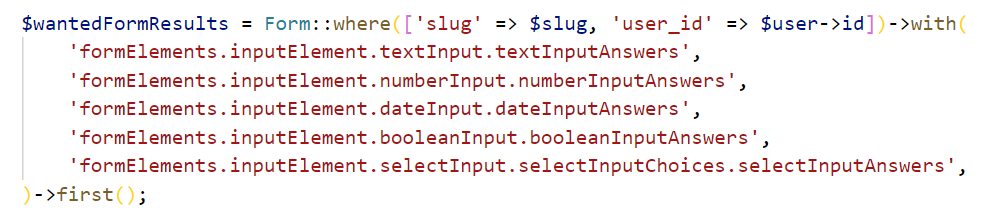
\includegraphics[width=0.9\textwidth]{img/vraceni_vsech_vysledku.png}
				\caption{Ukázka části kódu metody \textit{index} pro získání odpovědí na formulář}
				\label{fig:vraceni_vsech_vysledku}
			\end{figure}
			
			\subsubsubsection{Vrácení veřejných výsledků}
			Metoda s názvem \textit{publicIndex} slouží k vypsání všech odpovědí na formulář. Tento výpis je dostupný jen v případě, že majitel formuláře tuto funkci aktivoval (popsáno v sekci \ref{sec:form_publish_results}) - poté jsou vybrané výsledky dostupné pro kohokoliv. 
			
			Tato metoda funguje velmi podobně jako metoda \textit{index} popsaná v sekci \ref{sec:form_comp_private_index}. Oproti zmíněné metodě nekontroluje přihlášení uživatele, ale zda jsou výsledky dotazovaného formuláře nastaveny jako veřejné. Z podstaty věci také omezuje viditelnost vybraných otázek na základě hodnoty \textit{has\_public\_results}, kterou musí disponovat všechny otázky - pokud je nastavena na \textit{false}, tak je otázka z výstupního setu odebrána. Pokud jsou všechny nastaveny jako skryté, odesílá se stejný stavový kód jako při situaci, kdy neexistuje žádná odpověď na formulář. Jinak se tato metoda oproti zmíněné neliší.
			
			\subsubsubsection{Export výsledků}\label{sec:form_comp_export}
			Metoda s názvem \textit{export} je určena k exportování všech odpovědí do souboru formátu MS Excel (s příponou .xlsx). Tato data mají sloužit při správném nastavení formuláře a jeho odpovědí např. ke korelační analýze (především u škálových typů otázek). K tomuto úkonu je použit přídavný balíček \uv{maatwebsite/excel} (především třídu \textit{Excel}), který po předání příslušných dat celý exportní proces obstarává (viz sekce \ref{sec:exports}).
			
			Metoda funguje tak, že nejprve volá metodu \textit{index} (popsána v sekci \ref{sec:form_comp_private_index}), které předává identifikátor formuláře z uživatelského požadavku. Poté, pokud je ze zmíněné metody navrácen objekt formuláře (tzn. že celý proces proběhl úspěšně - byla předána platná kolekce odpovědí), jsou příslušná data předána metodě \textit{download} na statické třídě \textit{Excel}, která vygeneruje příslušný soubor. Pokud je z metody \textit{index} vrácen jen stavový kód, tak je uživateli předán společně s příslušnou chybovou hláškou.
			
			Samotný export dat je proveden tak, že se zmíněné metodě \textit{download} předá instance objektu, která zaobaluje předaná data k exportu a definuje, jak budou v souboru sázeny. Metoda \textit{download} poté vytvoří soubor, který je poslán uživateli. Instance objektu je tvořena ze třídy \textit{FormCompletionsExport}, která byla k tomuto účelu připravena - implementuje rozhraní \textit{FromArray} (z balíčku pro export) a obsahuje příslušnou metodu \textit{array}, která vybraná data zpracovává a vrací ve formě pole polí (reprezentuje sloupce a řádky v tabulce). Metoda určuje formát dat takto:
			
			\begin{itemize}
				\item Na prvním řádku v první buňce (roh tabulky) je umístěn samotný název formuláře.
				\item Na druhém řádku je nejprve definován sloupec \textit{Completion ID} (ten obsahuje ID pro každou zaznamenanou odpověď - jedná se o \textit{id} databázového objektu pro vyplnění formuláře viz sekce \ref{sec:form_completions}). Poté jsou sázeny jednotlivé otázky formuláře.
				\item Na dalších řádcích jsou vypsána data z odpovědi - tzn. na prvním místě ID vyplnění formuláře, poté příslušná odpověď pod příslušnou otázkou.
			\end{itemize}
		
			\begin{figure}[h]
				\centering
				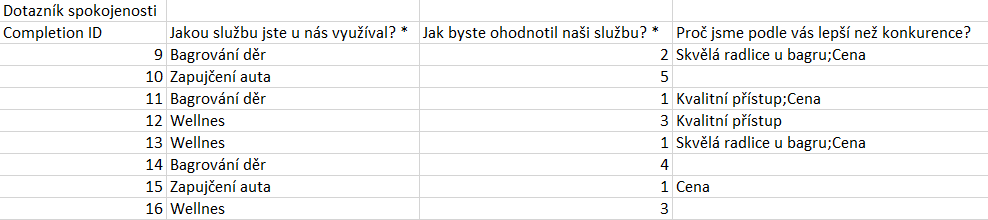
\includegraphics[width=0.95\textwidth]{img/export_excel.png}
				\caption{Ukázka vyexportovaných dat (pro potřeby této práce upraveno)}
				\label{fig:export_excel}
			\end{figure}
		
			Zpracování odpovědí nejprve probíhá tak, že se shromáždí všechna ID vyplnění formuláře pro požadovaný formulář - tím se vytvoří připravené \uv{chlívečky} pro odpovědi (jednorozměrné pole), které jsou od sebe oddělené právě pomocí ID vyplnění formuláře (co \textit{chlíveček}, to řádek s odpovědmi). Dále se na první index \uv{chlívečku} umístí samotné ID vyplnění. Poté se prochází jednotlivé odpovědi, které se postupně ukládají do zmíněných \uv{chlívečků}, přičemž je dbáno na to, aby se odpovědi ukládaly pod správné otázky. U otázek s možnostmi odpovědí v případě multiple-choice jsou data rozdělována středníkem. Pokud je otázka nepovinná a nebyla zodpovězena, buňka ve výstupu bude prázdná. 
			
			Nakonec se otázky rozmístěné do \uv{chlívečků} ještě upraví (tzn. kde se nachází logické hodnoty \textit{true} nebo \textit{false}, tam je umístěn textový ekvivalent \uv{true} nebo \uv{false}). Podobná úprava probíhá i u samotných otázek v 2. řádku tabulky (pokud je otázka povinná, je jí na konec přidán znak hvězdičky \uv{*}).
			
		\subsubsection{Interakce s uživateli}
		Tato část popisuje veškerou administrativu nad uživatelskými účty. Nutno zmínit, že v projektu byly pro tyto účely použity nativní materiály a funkce Laravelu (např. model uživatele, migrace tabulky uživatelů a validační funkce). V rámci validačních funkcí zde nebudou popsány stavové kódy, které při chybě vracejí, jelikož se jedná o funkcionalitu spravovanou přímo frameworkem Laravel.
		
			\subsubsubsection{Registrace uživatele}\label{sec:user_register}
			Metoda \textit{register} slouží k vytvoření nového uživatelského účtu.
			
			V rámci funkčnosti metoda nejdříve přijme požadavek od uživatele, ve kterém očekává určité parametry (přezdívka uživatele, email, heslo a potvrzení hesla). Pokud tyto parametry dostane a jsou platné (tzn. že splňují požadavky jako že se jedná o platné textové hodnoty, že email musí být u uživatele unikátní a že je heslo alespoň 8 znaků dlouhé), vytvoří se hash hesla (to je zašifrováno pomocí funkce \textit{bcrypt}) a všechna data o uživateli se uloží do databáze. 
			
			\subsubsubsection{Přihlášení uživatele}
			Metoda \textit{login} slouží k přihlášení uživatele k uživatelskému účtu. 
			
			Funkce funguje tak, že nejprve (podobně jako v metodě \textit{register} v sekci \ref{sec:user_register}) zvaliduje příchozí data (zde email a heslo) a až poté, co se ověří, že jsou údaje platné (pomocí statické třídy \textit{Auth}), se odesílá objekt s daty o přihlášeném uživateli.
			
			\subsubsubsection{Odhlášení uživatele}
			Metoda \textit{logout} slouží k odhlášení uživatele - tedy k invalidování relace. Obsahuje jen volání metody \textit{logout} na statické třídě \textit{Auth}, která zařizuje veškerou administrativu nad přihlášenými uživateli a tedy i nad tímto úkonem.
			
			\subsubsubsection{Vrácení informací o uživateli}
			Metoda \textit{show} přihlášenému uživateli vrátí data o jeho účtu resp. jeho osobní údaje jako je např. přezdívka nebo email.
			
			Funguje tak, že pokud je uživatel přihlášen, jsou jednoduše vrácena jeho osobní data z databáze. Pokud není přihlášen, je vrácen stavový kód 401.
			
			\subsubsubsection{Vymazání účtu uživatele}
			Metoda \textit{destroy} slouží k odstranění uživatelského účtu na základě požadavku vlastníka účtu. Vlastník k tomuto úkonu samozřejmě musí být přihlášen.
			
			Jelikož k tomuto úkonu musí být předáno současné heslo k účtu, je prvně kontrolováno právě to resp. jestli se jedná o validní textový řetězec. Poté je zjišťováno, zda je vůbec nějaký uživatel přihlášen (pokud není, je vrácen stavový kód 400). Pokud ano, je kontrolováno, zda se heslo shoduje s heslem v databázi (pokud ne, je vrácen stavový kód 400). Pokud se hesla shodují, je uživatel z databáze smazán.
			
			\subsubsubsection{Změna hesla}
			Metoda \textit{changePassword} slouží ke změně hesla za předpokladu, že uživatel stávající heslo zná.
			
			V rámci průběhu celého úkonu metody, prvně se kontroluje, zda je vůbec nějaký uživatel přihlášen. Pokud není, je vrácen stavový kód 401. Pokud ale přihlášen je, tak nejprve dochází k validaci dat (podobně jako v sekci \ref{sec:user_register}). Dále se kontroluje, zda je původní heslo shodné s předaným původním heslem, zda není staré a nové heslo stejně a zda je nové heslo shodné s potvrzením tohoto hesla. Pokud všemi kontrolami projde, dochází k vytvoření nového hashe hesla a ten přepisuje starý hash uživatele.
			
			\subsubsubsection{Resetování zapomenutého hesla uživatele}
			Tento proces je obhospodařován dvěma metodami - \textit{forgotPassword} a \textit{resetPassword}. Celý proces resetování hesla probíhá tak, že uživatel odešle požadavek na metodu \textit{forgotPassword}, která mu na jeho email pošle odkaz k resetování hesla - ten vede na stránku, kde si zvolí nové heslo. Poté, co heslo vyplní, odesílá požadavek na metodu \textit{resetPassword}, která heslo za splnění všech podmínek (tj. validace dat a správnost obnovovacího tokenu) změní. 
			
			Metoda \textit{forgotPassword} tedy v požadavku přijímá jen email, který je nejprve validován. Poté je na něj odeslán odkaz k resetování hesla. Pokud se odeslání nezdaří, je vrácen stavový kód 400.
			
			K metodě \textit{resetPassword} je přistupováno právě z odkazu poslaného pomocí metody \textit{forgotPassword}. Metoda \textit{resetPassword} přijímá ověřovací token předaný v odkazu v emailu, samotnou emailovou adresu a heslo s potvrzením. Pokud jsou předaná data validní, je vygenerován nový hash hesla, který přepíše stávající hash. Pokud se při resetování hesla vyskytne chyba, je vrácen stavový kód 400.
			


\section{Frontend}\label{sec:impl_frontend}
Frontendová část tohoto projektu zajišťuje především komunikaci mezi uživatelem a serverem pomocí prostředí, díky kterému je tato komunikace snazší a obecně přívětivější. Serverová část očekává příchozí požadavky od této části na cesty, které byly už definovány (viz sekce \ref{sec:routes}).

V rámci této implementace (a z podstaty využitých technologií) probíhá komunikace s API (viz sekce \ref{sec:impl_backend}), které se tato část snaží poskytovat validní data. Slovo \uv{snaží} je zmíněno proto, jelikož se na ni v reálném světe nemůžeme úplně spoléhat - frontendovou část může uživatel s dostatečnými znalostmi a zkušenostmi modifikovat, čímž může i změnit způsob komunikace se serverem. To ale neznamená, že na ní nemůže probíhat jakákoliv validace a kontrola dat - frontend pro správnou funkčnost celé aplikace musí serveru ve výchozím (uživatelem nezměněném) stavu backendu poskytovat validní data - backend je ale musí preventivně validovat taky.

Uživatelské prostředí musí být připraveno tak, aby bylo příjemné k užívání a ergonomické. Zároveň by nemělo být nějak složité a přehlcené ovládacími prvky, což by mohlo uživatele od používání aplikace odradit. Dále by toto prostředí mělo uživatele \uv{vést} úkonem, který chce uživatel provést - tzn. pokud zadává neplatná data, tak ho upozornit a rozhodně počkat na opravu dat před odesláním požadavku na server. Uživatelské prostředí, které v rámci tohoto projektu vzniklo, je určeno primárně pro vykreslování ve webovém prohlížeči.

V následující části jsou popsány jednotlivé frontendové komponenty a principy, díky kterým může celá aplikace fungovat.
	
	\subsection{Obecná struktura VueJS aplikace}\label{sec:obecna_str_vuejs}
	Nejprve je nutné rozebrat obecnou strukturu VueJS projektu.
	
	\begin{figure}[H]
		\centering
		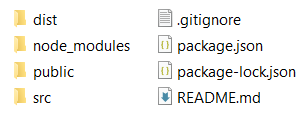
\includegraphics[width=0.6\textwidth]{img/vuejs_struktura.png} 
		\caption{Obecná struktura nově vygenerovaného VueJS projektu}
		\label{fig:vuejs_str}
	\end{figure}

	Jak můžeme na obrázku \ref{fig:vuejs_str} vidět, celý projekt je složen z mnoha složek a souborů. Podrobný rozbor všech souborů a složek není předmětem této práce, proto jsou nejdůležitější zmíněné části popsány níže jen obecně.
	
	\begin{itemize}
		\item Složka \textit{dist} obsahuje zkompilovaný kód aplikace
		\item Složka \textit{node\_modules} obsahuje závislosti a soubory přídavných balíčků NPM (viz sekce \ref{sec:npm}), které aplikace používá
		\item Složka \textit{public} obsahuje obecně veřejné soubory (např. favicon)
		\item Složka \textit{src} obsahuje všechny soubory se zdrojovým kódem, ze kterých se poté tvoří zkompilovaný kód celé aplikace
		\item Soubor \textit{package.json} obsahuje informace o přídavných balíčcích spravovaných pomocí NPM (viz sekce \ref{sec:npm})
	\end{itemize}

	*cite https://5balloons.info/project-tour-of-vue-cli-app/*
	*cite https://stackoverflow.com/questions/22842691/what-is-the-meaning-of-the-dist-directory-in-open-source-projects*
	
	Popsaná struktura výše je standardní pro oddělenou frontendovou aplikaci. To v implementaci tohoto projektu ale neplatí, jelikož je frontend přímo zaintegrován v Laravel projektu (viz sekce \ref{sec:strukura_laravel}). Jsou zde tyto rozdíly:
	
	\begin{itemize}
		\item Složka \textit{src} je nahrazena složkou \textit{js} ve složce \textit{resources}
		\item Složka \textit{public} je umístěna v kořenovém adresáři Laravel projektu a je sloučena se složkou \textit{dist}
		\item Složka \textit{node\_modules} společně se souborem \textit{package.json} je také umístěna v kořenovém adresáři Laravel projektu
	\end{itemize}
	
	Celkovou administrativu nad celým Vue projektem poté zajišťuje modul Laravel Mix podle konfiguračního souboru webpack.mix.js. Ten je také umístěn v kořenovém adresáři projektu. *cite https://laravel-mix.com/docs/6.0/vue* Díky celému tomuto přístupu může backend i frontend běžet jako jedna aplikace na jedné doméně.
	
	Jak již bylo zmíněno, zdrojový kód, tedy nejdůležitější část frontendové aplikace, leží standardně ve složce \textit{src} - v tomto projektu ve zmíněné složce \textit{js}. Oproti běžné samostatné Vue aplikaci je zde (ve složce \textit{js}) největší rozdíl v pojmenování souborů - soubor \textit{main.js} byl přejmenován pro potřeby Laravelu na \textit{app.js}. Také se navíc v této složce nachází Laravelem vygenerovaný soubor bootstrap.js pro další konfiguraci při kompilaci. Nakonec byla kvůli nevyužití odebrána složka \textit{assets} a pro další účely přidána složka \textit{apis} (viz obrázek \ref{fig:zdroj_kod_vue_rozdily}).
	
	\begin{figure}[h]
		\centering
		\subfloat[\centering]{{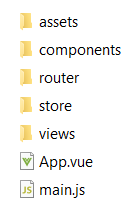
\includegraphics[height=5cm]{img/zdroj_kod_vue/src.png} }}
		\qquad
		\subfloat[\centering]{{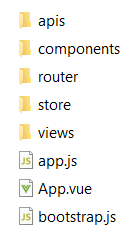
\includegraphics[height=5cm]{img/zdroj_kod_vue/js.png} }}
		\caption{Porovnání obsahu složek \textit{src} (a) a \textit{js} (b)}
		\label{fig:zdroj_kod_vue_rozdily}
	\end{figure}

	Každý soubor a složka ve zmíněném adresáři \textit{js} má určitý význam. Ty jsou představeny níže (soubor bootstrap.js byl již popsán výše). Další rozbor jednotlivých souborů ve zmíněných složkách je obsažen v dalších sekcích této práce.
	\begin{itemize}
		\item Složka \textit{apis} obsahuje prostředky pro komunikaci s API (tedy s backendem)
		\item Složka \textit{components} obsahuje všechny komponenty, které jsou využívány v celé aplikaci
		\item Složka \textit{router} obsahuje prostředky pro přesměrovávání a definování cest ve frontendové aplikaci
		\item Složka \textit{store} obsahuje nástroje pro držení dat ve webovém prohlížeči
		\item Složka \textit{views} obsahuje veškeré pohledy, na které se můžeme pomocí definované cesty dostat
		\item Soubor \textit{app.js} je kořenový soubor aplikace shromažďující všechny reference na ostatní soubory (zabaluje celou aplikaci)
		\item Soubor \textit{App.vue} je kořenová šablona, která přijímá pohledy na základě cesty, které poté vykresluje (tvoří aplikační kostru HTML)
	\end{itemize}

		\subsubsection{Souhrn využitých balíčků}\label{sec:fe_packages}
		Pro přehlednost je zde vytvořena kapitola shrnující vybrané externí balíčky, které byly do frontendové části přidány, a jejich základní účel a funkcionalita.
		
		\begin{itemize}
			\item Balíček \uv{@braid/vue-formulate} (dále jako VueFormulate) je použit pro veškeré formulářové prvky. Kromě zprostředkování hotových komponent pro jednotlivé elementy formuláře také nabízí např. validaci dat.
			\item Balíček \uv{vue-chartjs} (zastřešující populární balíček \uv{chart.js}) je použit pro grafické vyobrazení dat ve formě grafů.
			\item Balíček \uv{randomcolor} je použit pro generování náhodných barev (využito u grafů k dynamickému rozlišení dat)
			\item Balíček \uv{uuid} je použit pro generování unikátního identifikátoru (především funkce \textit{uuidv4}, např. u vytváření formuláře k označování vytvořených otázek)
			\item Balíček \uv{vue-js-modal} je použit k vytváření a správě modálních oken.
			\item Balíček \uv{vue-toasted} je použit pro zobrazování zpráv o průběhu různých činností (např. zobrazení chybových hlášek).
		\end{itemize}
	
		Dále frontend obsahuje reference na automaticky přidané balíčky, které nejsou předmětem této práce. Lze z nich ale vyjmout např. \uv{vuex} (správa držení dat v prohlížeči), \uv{vue-router} (správa cest mezi jednotlivými částmi aplikace - směrovač) či \uv{axios} (komunikace s API).
	
	\subsection{Komponenty}
	Komponenty jsou v podstatě \uv{díly k složení celé aplikace}. Díky nim nemusíme např. stránku pro vytvoření formuláře psát do jednoho nepřehledného a obrovského souboru, ale můžeme tento kód rozdělit. Výhodou také je, že když budeme tento komponentový styl zápisu kódu dodržovat, lze jeho části v jiných místech opětovně využít - předcházíme tím redundantnímu kódu, který zbytečně znepřehledňuje celý projekt. Všechny zmíněné komponenty jsou zapsány v souborech s koncovkou \textit{.vue} a disponují stejným jménem jako samotný soubor.
		
		\subsubsection{Základní komponenty} %Header, Loading, teor. App.vue
		Mezi základní komponenty jsou řazeny především ty, jejichž použití se opakuje v aplikaci nejčastěji - tedy \textit{Header} a \textit{Loading}. 
		
		Komponenta \textit{Header} slouží k vykreslení horního navigačního panelu s nabídkou dalších funkcionalit, který na základě přihlášení uživatele mění svůj obsah. Pokud není nikdo přihlášen, nabídka nabízí odkazy na přihlášení či registraci. Pokud se uživatel přihlásí, může se odsud dostat na stránku svého profilu, na vytvoření nového formuláře nebo se odhlásit ze svého účtu.
		
		Komponenta \textit{Loading} obsahuje jednoduchou animaci, která symbolizuje průběh načítání. Je využita v částech komponent a pohledů, kde je očekáván např. příjem nějakých dat z backendu, na který se musí čekat. Uživateli má vyobrazovat, že v aplikaci probíhá nějaká činnost.
		
		Dále zde lze zmínit i komponentu \textit{App} z kořenového adresáře frontendu, která již byla popsána v sekci \ref{sec:obecna_str_vuejs}. Lze dodat, že se v ní kromě předaných pohledů nachází i reference na komponentu \textit{Header} - ta musí být z podstaty věci vykreslena na všech cestách.
		
		\subsubsection{Komponenty elementů formuláře} %Elements, FormElement...*
		Tyto komponenty představují jednotlivé otázky a k ním příslušný vstup definovaný typem (pokud se nejedná o element nové stránky). Existují zde interaktivní komponenty elementů (použity např. ve vyobrazení celého formuláře k vyplnění) nebo komponenty statické (použity např. ve vyobrazení jednotlivých otázek při vytváření formuláře).
		
		Interaktivní komponenty elementů formuláře nalezneme v podsložce \textit{Elements} - zde se nachází tyto komponenty: \textit{BooleanInput}, \textit{DateInput}, \textit{NumberInput}, \textit{SelectInput} a \textit{TextInput} (vycházející z typů ze sekce \ref{sec:form_inputs_types}). Všechny tyto komponenty jsou si navzájem velmi podobné. Všechny využívají komponenty z balíčku \uv{VueFormulate}: \textit{FormulateInput} pro vykreslení samotné otázky a vytvoření vstupního pole podle datového typu pro odpověď (např. pro text je vygenerována oblast, do které lze vkládat textový řetězec) a \textit{FormulateErrors} pro výpis validační chyby (např. pokud má mít vkládaný text délku maximálně deset znaku a do oblasti vstupu je vložen text delší, tak se objeví chybové hlášení pod otázkou). V logické části jsou si taktéž všechny komponenty podobné - při jejich inicializaci se na základě přijmutích dat nastaví validační pravidla pro vstup a ID otázky, ke které samotná komponenta patří.
		
		Tyto interaktivní komponenty jsou poté zabaleny do dalších komponent. Komponenta \textit{FormElement} na základě příchozích dat (tj. typ otázky) vrací rodičovské komponentě \textit{FormElementsComponent} příslušný element formuláře rozebraný v předchozím odstavci. Zmíněná rodičovská komponenta poté figuruje především při vykreslování celého formuláře - má za úkol vykreslovat veškeré otázky formuláře s funkcí stránkování. Při inicializaci této komponenty se otázky nejprve rozdělí do příslušných polí, které představují stránky, na základě výskytu elementu nové stránky (tzn. pokud se při procházení všech elementů formuláře najde element nové stránky, tak je vytvořeno nové pole, do kterého se přesouvají další otázky). Po vzniku těchto polí představující stránky dojde k jejich vykreslení pomocí zmíněné komponenty \textit{FormElement}. Stránkování je zde zajištěno pomocí skrývání a odkrývání jednotlivých stránek pomocí CSS stylů ovládaných příslušnými tlačítky - takto to je řešeno kvůli udržení dat při přesunu na další stránku (nutné opatření kvůli zmíněnému balíčku k tvoření formulářových prvků).
		
		V rámci statických komponent zde existuje komponenta \textit{FormElementControl}. Ta slouží k vykreslování reprezentace otázek nebo elementu nové stránky v pohledech vytváření nebo úpravě formuláře. Jedná se o komponentu, která na základě předaného typu elementu (tj. otázka s příslušným typem nebo nová stránka) vrací příslušnou reprezentaci elementu (např. v případě textového vstupu vyobrazení textového pole, do kterého nelze vyplňovat, a samotné otázky). Při kliknutí na element otázky se objeví modální okno pro úpravu vybrané otázky - toto modální okno je popsáno dále v práci. U elementu nové stránky toto provést nelze, proto je zde připraven jen prokliknutelný text \uv{Remove}, který vysílá specifickou událost do rodičovské komponenty, která ho používá (slouží k odebrání elementu).
	
		\subsubsection{Modální okna} %Modals
		Zmíněné komponenty představují předpis vykreslení pro modální okna spravovaná balíčkem \uv{vue-js-modal}. Na jejich funkčnosti závisí několik pohledů. Tyto komponenty se nachází v podsložce \textit{Modals} - zde existují ještě další tři podsložky pojmenované podle oblasti, ve které jsou používány. Ty poté obsahují příslušné soubory komponent. Jedná se tedy o tyto složky: \textit{CreateForm}, \textit{FormResults}, \textit{FormReview}. 
		
			\subsubsubsection{Manipulace s elementy formuláře}
			První adresář \textit{CreateForm} obsahuje příslušné komponenty modálních oken a podkomponenty využívané především v pohledu vytváření formuláře. Později byly tyto komponenty využity i v pohledu pro úpravu formuláře - název tohoto adresáře se ale neměnil. Adresář obsahuje komponenty modálních oken \textit{ItemModal} a \textit{SelectChoiceModal}.
			
			Komponenta \textit{ItemModal} slouží k samotné tvorbě nového elementu nebo úpravě stávajícího elementu otázky ve formuláři - to je možné pomocí manipulace s dočasným úložištěm dat \textit{createFormStore} (viz \ref{sec:data_prohlizec_form}), se kterým se pracuje např. v rodičovském pohledu pro vytváření formuláře. K manipulaci s daty využívá příslušné metody inicializovaného úložiště.
			
			Celé modální okno je zobrazeno na základě vyžádání rodičovského prvku (např. pohledu pro vytvoření formuláře) a je tvořeno zejména komponentou \textit{FormulateForm} (z balíčku \uv{VueFormulate}), ve které jsou vnořeny všechny ovládací prvky (tvořené komponentami \textit{FormulateInput} a \textit{FormulateErrors}) - ty shromažďují veškeré informace o elementu otázky - tedy typ odpovědi na otázku (např. text nebo číslo), samotnou otázku, zda je otázka povinná a další validační pravidla, která jsou vázána na typ otázky (tato pravidla vychází ze sekce \ref{sec:form_inputs_types}). Ovládací prvky dalších validačních pravidel jsou další samotné komponenty připojované do modálního okna - každý typ otázky má pro tyto účely svou podkomponentu (jedná se o \textit{DateItem}, \textit{NumberItem}, \textit{SelectItem} a \textit{TextItem} ve stejné složce). Tyto prvku mohou být už předvyplněny v situaci, kdy je upravován existující element (komponenta může přijímat vstupní hodnoty). Data jsou poté na základě stisknutí příslušného tlačítka (např. s účelem vytvoření nového elementu s textem \uv{Create}) z modálního okna předána příslušné metodě úložiště, která si data sama zpracuje.
			
			Známou komplikací je samozřejmě zpracování otázek s možnostmi odpovědi. K těmto účelům je v komponentě \textit{SelectItem} vnořena další podkomponenta \textit{SelectChoicesComponent}. Tato komponenta poskytuje administrativu nad možnostmi odpovědi - k tomu používá vlastní dočasné úložiště \textit{createFormChoicesStore}, které má stejné metody jako již zmíněné úložiště \textit{createFormStore} (data z celé této komponenty samozřejmě podléhají i manipulaci s daty rodičovské komponentě \textit{ItemModal}). V komponentě jsou kromě tlačítka pro přidání možnosti odpovědi vykreslovány možnosti odpovědi. Ty lze samozřejmě modifikovat - při kliknutí na ně se zobrazí další modální okno \textit{SelectChoiceModal}, ve kterém ji lze upravit příslušné hodnoty (toto okno je používáno i k přidávání těchto možností). Toto okno poté data předává zmíněnému poskytnutému úložišti. Zajímavou funkcí, kterou lze u \textit{SelectChoicesComponent} zmínit, je hlídání hodnoty \textit{hasHiddenLabel} pocházející z rodičovské komponenty (ta značí, zda možnosti odpovědi mají skrytý popisek - tj. škála) - pokud je tato hodnota změněna z \textit{true} na \textit{false}, tak jsou automaticky tyto skryté popisky odstraněny. V opačném případě komponenta automaticky očísluje možnosti odpovědi čísly 1,2,3,...
			
			\subsubsubsection{Výsledky formuláře}
			Dalším adresářem je \textit{FormResults} obsahující pouze jedno modální okno. To je využito zejména v pohledu pro zobrazení výsledků formuláře. Toto okno je znovu tvořeno především prvky z balíčku \uv{VueFormulate}. 
			
			Před inicializací přijímá všechny otázky formuláře, hodnotu vyjadřující zda je formulář už zveřejněn a identifikátor formuláře. Poté, na základě přijatých dat, vypisuje jeho současný stav a možnosti, co lze s formulářem provést. Klíčová je hodnota vyjadřující zda jsou už výsledky veřejné - pokud se rovná \textit{false}, je zobrazeno jen prázdné zaškrtávací políčko vyjadřující, že výsledky zveřejněny nejsou. Pokud se hodnota rovná \textit{true}, jsou vypsány i všechny otázky, u kterých lze označit, která z nich bude veřejně viditelná. Zmíněnou hodnotu můžeme pomocí zaškrtávacího políčka samozřejmě měnit - s tím se i dynamicky změní rozložení okna. Poté, co navolíme příslušné parametry a klikneme na tlačítko pro uložení nastavení, je na server poslán požadavek s příslušnými údaji. Ten je zpracován metodou \textit{publishResults}, která je popsána v sekci \ref{sec:form_publish_results}. Po úspěšném provedení činnosti se okno zavírá a celá stránka je přenačtena.
			
			\subsubsubsection{Manipulace s celým formulářem}
			Posledním adresářem je \textit{FormReview}. Ten obsahuje dvě modální okna použitá v pohledu pro zobrazení souhrnu informací o formuláři. Jedná se o komponenty \textit{FormAccessibilityModal} a \textit{FormDuplicationModal}.
			
			Komponenta \textit{FormAccessibilityModal} slouží k úpravě přístupnosti formuláře. Je také tvořena především komponentami z balíčku \uv{VueFormulate} a ke svému správnému chodu potřebuje při vytvoření nejprve dostat hodnotu vyjadřující současnou přístupnost (zda je formulář veřejný nebo privátní) a identifikátor formuláře - pokud se jedná o privátní formulář, musí být předány i emaily, na které byla už zaslána pozvánka. Na základě těchto dat je vykresleno příslušné rozložení modálního okna - toto rozložení lze měnit na základě změny hodnoty vyjadřující přístupnost. Pokud je zmíněná hodnota \textit{false}, zobrazí se jen související prázdné zaškrtávací políčko. Pokud se ale rovná \textit{true}, zobrazují se zde i další dva ovládací prvky. V prvním lze vidět emaily, na které již byla zaslána pozvánka - ty lze pro zneplatnění pozvánky označit. V druhém můžeme zase přidat emaily, na které bude poslána nová pozvánka k vyplnění formuláře. Nakonec (po kliknutí na tlačítko vyjadřující provedení změny) se příslušná data pošlou na server. Ta jsou zpracována metodou \textit{updateAccess}, která je popsána v sekci \ref{sec:form_accessibility}. Modální okno se poté zavře a stránka je přenačtena.
			
			Druhá komponenta \textit{FormDuplicationModal} nám umožňuje duplikovat vybraný formulář. I toto modální okno je tvořeno komponentami z balíčku \uv{VueFormulate} a při inicializaci očekává základní data o formuláři - tedy jeho název, popisek, datum zveřejnění, datum ukončení zveřejnění a zda se jedná o formulář veřejný či privátní (u privátního také emaily, které dostali pozvánku). Tato data jsou dočasně uložena v úložišti \textit{duplicateFormStore}, které je popsáno v sekci \ref{sec:data_prohlizec_form}. Tyto údaje lze libovolně měnit - pokud jsou zadány neplatné hodnoty (např. datum zveřejnění je dále v čase než datum ukončení zveřejnění), tak nás okno bude informovat příslušným upozorněním. Poté, co klikneme na příslušné tlačítko pro duplikaci formuláře, je odeslán na server požadavek, který je vyřízen metodou \textit{duplicateWithAuth}, jež je popsána v sekci \ref{sec:form_dupl}. Po tomto úkonu je modální okno zavřeno a stránka přenačtena.
		
		\subsubsection{Komponenty pro zobrazení výsledků} %ResultComponents
		Dalšími komponentami, které jsou zde popsány, jsou komponenty pro grafické znázornění dat v pohledu pro zobrazení výsledků formuláře (pro vyobrazení dat ve formě grafů zde byl použit balíček \uv{vue-chartjs}). Nachází se v adresáři \textit{ResultComponents}, který obsahuje komponenty \textit{DetailedResultsTable}, \textit{ResultComponent} a \textit{ResultRender}. Také se zde nachází podsložka \textit{Views}, ve které lze najít předpřipravené podkomponenty pro konkrétní styl vykreslení dat - \textit{Bar} pro vykreslování sloupcových grafů, \textit{List} pro vykreslování jednoduché tabulky stylem klíč/hodnota (resp. ID odpovědi/odpověď) a \textit{Pie} pro vykreslování koláčových grafů. Tyto podkomponenty jsou poté předávány dál pomocí zmíněné komponenty \textit{ResultRender}, která je vrací na základě předaného typu a dat (tzn. výsledky z otázek s možnostmi odpovědi nebo z otázek Ano/Ne jsou zobrazovány jako grafy - lze si mezi zmíněnými styly grafu po načtení vybrat, ostatní jako zmíněná tabulka).
		
		Popsaná komponenta \textit{ResultRender} je poté využita ve zmíněné komponentě \textit{ResultComponents}. Pro správnou funkcionalitu komponenta \textit{ResultComponents} musí pro získání příslušného vyobrazení dat samozřejmě předaná data zpracovat do validního formátu a poté je poskytnout komponentě \textit{ResultRender}. Nakonec zmíněná rodičovská komponenta \textit{ResultComponents} přidá k vyobrazení dat (např. ve formě grafu) samotnou otázku a celý obsah je předán do pohledu pro zobrazení výsledků.
		
		Nelze opomenout komponentu \textit{DetailedResultsTable}, která slouží jako alternativní zobrazení všech výsledků formuláře. (ve výchozím nastavení se zobrazují data ve zmíněných grafech nebo v tabulce pro každou otázku). V podstatě data zobrazuje v podobném formátu, jako jsou vysázeny při exportu dat (tzn. v tabulce viz sekce \ref{sec:form_comp_export}). Oproti exportu se vyobrazení dat liší v tom, že v buňkách, kde není žádná hodnota (\textit{null}), tam je umístěn znak pomlčky (\uv{-}).
		
		\subsubsection{Komponenta karty formuláře}
		Jednoduchá komponenta, kterou nebylo možné zařadit mezi ostatní výše, s názvem \textit{FormCard} slouží jako předpis pro vykreslování karty formuláře. Ta je použita v pohledu úvodní stránky v případě, že je uživatel přihlášen a že už nějaké formuláře vlastní. Po kliknutí na kartu se přihlášený uživatel dostane na pohled se zobrazením souhrnu informací o požadovaném formuláři. Sama o sobě karta zobrazuje název a popisek formuláře či data spuštění a ukončení zveřejnění formuláře.
		
	\subsection{Komunikace s Laravel API}
	
	
	\subsection{Směrovač} %%Router
	
	\subsection{Držení dat v prohlížeči} %% Store
	
	
		\subsubsection{Přihlášení uživatele}
		
		
		\subsubsection{Data pro manipulaci s formuláři}\label{sec:data_prohlizec_form}
		
	
	\subsection{Pohledy}
		
		\subsubsection{Přihlašování a profil}
		
		\subsubsection{Domovská stránka}
		
		\subsubsection{Formulář}
		
		\subsubsection{Tvorba formuláře}
		
		\subsubsection{Úprava formuláře}
		
		\subsubsection{Souhrn informací o formuláři}
		
		\subsubsection{Výsledky formuláře}
		
		\subsubsection{Ostatní pohledy}
		%% not found, about

\chapter{Závěr}
Vznikla ...


Lorem ipsum haf baf haf. Co lze zlepšit - update formuláře!




\begin{thebibliography}{50}

\bibitem{GoogleForms1}
Google Forms: Free Online Form Creator | Google Workspace. \textit{Google} [online]. [cit. 2022-01-15]. Dostupné z: https://www.google.com/forms/about/

\bibitem{GoogleForms2}
DEMAREST, Abigail Abesamis. What are Google Forms? Everything you need to know about Google Workspace's online form builder. \textit{Business Insider} [online]. 2021, 22.1.2021 [cit. 2022-01-15]. Dostupné z: https://www.businessinsider.com/what-is-google-forms

\bibitem{MSForms1}
Microsoft Forms | Průzkumy, hlasování a kvízy. \textit{Microsoft Forms} [online]. [cit. 2022-01-30]. Dostupné z: https://www.microsoft.com/cs-cz/microsoft-365/online-surveys-polls-quizzes

\bibitem{MSForms2}
Microsoft Forms --- Užitečný nástroj, díky němuž se mnoho dozvíte. \textit{Microsoft Forms} [online]. 2021, 3.2.2021 [cit. 2022-01-30]. Dostupné z: https://manica.cz/microsoft-forms-uzitecny-nastroj-diky-nemuz-se-mnoho-dozvite/

\bibitem{Survio}
Dotazník zdarma: Vytvořit online dotazník. \textit{Survio®} [online]. [cit. 2022-01-30]. Dostupné z: https://www.survio.com/cs/

\bibitem{FEvsBE}
VERNEROVÁ, Sára. Front end vs. Back end - jaký je mezi nimi rozdíl?. \textit{Apitree} [online]. 2021, 12.9.2021 [cit. 2022-02-04]. Dostupné z: https://www.apitree.cz/blog/front-end-vs-back-end-jaky-je-mezi-nimi-rozdil

\bibitem{JS1}
JavaScript. \textit{Wikipedia} [online]. 2021, 16.12.2021 [cit. 2022-02-04]. Dostupné z: https://cs.wikipedia.org/wiki/JavaScript

\bibitem{JS2}
KOĎOUSKOVÁ, Barbora. JavaScript pro začátečníky: co to je a jak funguje. \textit{Rascasone} [online]. 2022, 28.01.2022 [cit. 2022-01-23]. Dostupné z: https://www.rascasone.com/cs/blog/co-je-javascript-pro-zacatecniky

\bibitem{VueJS1}
Introduction. \textit{Vue.js} [online]. [cit. 2022-01-23]. Dostupné z: https://vuejs.org/v2/guide/\#What-is-Vue-js

\bibitem{VueJSSyntax}
SFC Syntax Specification. \textit{Vue.js} [online]. [cit. 2022-01-23]. Dostupné z: https://v3.vuejs.org/api/sfc-spec.html\#custom-blocks

\bibitem{VueJS2}
Úvod do frameworku Vue.js. \textit{Vue manuál} [online]. [cit. 2022-01-23]. Dostupné z: https://vue.baraja.cz/uvod-do-vue

\bibitem{Bootstrap1}
The most popular HTML, CSS, and JavaScript framework for developing responsive, mobile first projects on the web. \textit{GitHub} [online]. [cit. 2022-01-30]. Dostupné z: https://github.com/twbs/bootstrap

\bibitem{Bootstrap2}
Bootstrap (front-end framework). \textit{Wikipedia} [online]. 2022, 2022 [cit. 2022-01-30]. Dostupné z: https://en.wikipedia.org/wiki/Bootstrap\_(front-end\_framework)

\bibitem{Bootstrap3}
About · Bootstrap v5.1. \textit{Bootstrap} [online]. [cit. 2022-01-30]. Dostupné z: https://getbootstrap.com/docs/5.1/about/overview/

\bibitem{NPM}
About npm. \textit{Npm Docs} [online]. [cit. 2022-03-03]. Dostupné z: https://docs.npmjs.com/about-npm

\bibitem{BE1}
ŠTRÁFELDA, Jan. Co je backend. \textit{Jan Štráfelda} [online]. [cit. 2022-01-30]. Dostupné z: https://www.strafelda.cz/backend

\bibitem{BE2}
Backend. \textit{Shoptet.cz} [online]. [cit. 2022-01-30]. Dostupné z: https://www.shoptet.cz/slovnik-pojmu/backend/

\bibitem{PHP1}
PHP: What is PHP?. \textit{PHP.net} [online]. [cit. 2022-02-22]. Dostupné z: https://www.php.net/manual/en/intro-whatis.php

\bibitem{PHP2}
PHP: What can PHP do?. \textit{PHP.net} [online]. [cit. 2022-02-22]. Dostupné z: https://www.php.net/manual/en/intro-whatcando.php

\bibitem{Laravel1}
Introduction. \textit{Laravel} [online]. [cit. 2022-01-30]. Dostupné z: https://laravel.com/docs/4.2/introduction

\bibitem{LaravelMVC}
How Laravel implements MVC and how to use it effectively. \textit{Pusher} [online]. 2018, 22.8.2018 [cit. 2022-01-31]. Dostupné z: https://blog.pusher.com/laravel-mvc-use/

\bibitem{LaravelEco}
Laravel Ecosystem Tools --- How Development Can be Faster and More Effective. \textit{ASPER BROTHERS} [online]. 2019, 20.4.2019 [cit. 2022-01-30]. Dostupné z: https://asperbrothers.com/blog/laravel-ecosystem-tools/

\bibitem{MVC}
ČÁPKA, David. MVC architektura. \textit{Itnetwork.cz} [online]. [cit. 2022-01-31]. Dostupné z: https://www.itnetwork.cz/navrh/mvc-architektura-navrhovy-vzor

\bibitem{Composer}
Introduction. \textit{Composer} [online]. [cit. 2022-03-03]. Dostupné z: https://getcomposer.org/doc/00-intro.md

\bibitem{Webhosting}
Webhosting. \textit{Wikipedia} [online]. 2021, 27.10.2021 [cit. 2022-01-30]. Dostupné z: https://cs.wikipedia.org/wiki/Webhosting

\bibitem{DO1}
SALEEM, Salman. What is DigitalOcean and why should you host apps on it?. \textit{The Official Cloudways Blog} [online]. 2021, 20.12.2021 [cit. 2022-01-30]. Dostupné z: https://www.cloudways.com/blog/what-is-digital-ocean/

\bibitem{DO2}
DigitalOcean Products | Designed for Developers, Built for Businesses. \textit{Digitalocean.com} [online]. [cit. 2022-01-30]. Dostupné z: https://www.digitalocean.com/products

\bibitem{DO3}
DigitalOcean App Platform: Build, Deploy and Scale Apps Quickly. \textit{Digitalocean.com} [online]. [cit. 2022-01-30]. Dostupné z: https://www.digitalocean.com/products/app-platform

\bibitem{Heroku1}
About Heroku. \textit{Heroku} [online]. [cit. 2022-01-30]. Dostupné z: https://www.heroku.com/about

\bibitem{Heroku2}
The Heroku product suite. \textit{Heroku} [online]. [cit. 2022-01-30]. Dostupné z: https://www.heroku.com/products

\bibitem{DBSummary}
What is a database?. \textit{Oracle | Cloud Applications and Cloud Platform} [online]. [cit. 2022-01-31]. Dostupné z: https://www.oracle.com/cz/database/what-is-database/

\bibitem{DBModel}
KUČEROVÁ, Helena. Databázový model. \textit{KTD: Česká terminologická databáze knihovnictví a informační vědy (TDKIV)} [online]. Praha: Národní knihovna ČR, 2003 [cit. 2022-02-04]. Dostupné z: \url{https://aleph.nkp.cz/F/?func=direct&doc\_number=000000091&local\_base=KTD}

\bibitem{HierarchDB}
KUČEROVÁ, Helena. Hierarchická databáze. \textit{KTD: Česká terminologická databáze knihovnictví a informační vědy (TDKIV)} [online]. Praha: Národní knihovna ČR, 2003 [cit. 2022-02-04]. Dostupné z: \url{https://aleph.nkp.cz/F/?func=direct&doc\_number=000000103&local\_base=KTD}

\bibitem{SitDB}
KUČEROVÁ, Helena. Síťová databáze. \textit{KTD: Česká terminologická databáze knihovnictví a informační vědy (TDKIV)} [online]. Praha: Národní knihovna ČR, 2003 [cit. 2022-02-04]. Dostupné z: \url{https://aleph.nkp.cz/F/?func=direct&doc\_number=000000128&local\_base=KTD}

\bibitem{RelacDB}
KUČEROVÁ, Helena. Relační databáze. \textit{KTD: Česká terminologická databáze knihovnictví a informační vědy (TDKIV)} [online]. Praha: Národní knihovna ČR, 2003 [cit. 2022-02-04]. Dostupné z: \url{https://aleph.nkp.cz/F/?func=direct&doc\_number=000000126&local\_base=KTD}

\bibitem{OOPDB}
MEHRA, Puran. What Are Object-Oriented Databases And Their Advantages. \textit{C\# Corner} [online]. 6.9.2019 [cit. 2022-02-04]. Dostupné z: https://www.c-sharpcorner.com/article/what-are-object-oriented-databases-and-their-advantages2/

\bibitem{DotazJazyk}
KUČEROVÁ, Helena. Dotazovací jazyk. \textit{KTD: Česká terminologická databáze knihovnictví a informační vědy (TDKIV)} [online]. Praha: Národní knihovna ČR, 2003 [cit. 2022-02-05]. Dostupné z: \url{https://aleph.nkp.cz/F/?func=direct&doc\_number=000000098&local\_base=KTD}

\bibitem{SQL}
BRITANNICA, The Editors of Encyclopaedia. SQL. \textit{Encyclopedia Britannica} [online]. 16.6.2021 [cit. 2022-02-05]. Dostupné z: https://www.britannica.com/technology/SQL

\bibitem{Transakce}
What is a Transaction? - Win32 apps. \textit{Microsoft} [online]. 2021, 1.7.2021 [cit. 2022-02-05]. Dostupné z: https://docs.microsoft.com/en-us/windows/win32/ktm/what-is-a-transaction

\bibitem{ACID}
IAN. What does ACID mean in Database Systems?. \textit{Database.Guide} [online]. 2016, 20.6.2016 [cit. 2022-02-05]. Dostupné z: https://database.guide/what-is-acid-in-databases/

\bibitem{PostgreSQL}
About. \textit{PostgreSQL} [online]. [cit. 2022-02-05]. Dostupné z: https://www.postgresql.org/about/

\bibitem{LaravelDir}
Directory Structure. \textit{Laravel} [online]. [cit. 2022-02-19]. Dostupné z: https://laravel.com/docs/8.x/structure

\bibitem{LaravelArtisan}
Artisan Console. \textit{Laravel} [online]. [cit. 2022-02-19]. Dostupné z: https://laravel.com/docs/8.x/artisan

\bibitem{ComposerpJSON}
Package.json. \textit{Npm Docs} [online]. [cit. 2022-02-19]. Dostupné z: https://docs.npmjs.com/cli/v8/configuring-npm/package-json
\bibitem{NPMpJSON}
Basic usage. \textit{Composer} [online]. [cit. 2022-02-19]. Dostupné z: https://getcomposer.org/doc/01-basic-usage.md

\bibitem{LaravelJSCSS}
JavaScript \& CSS Scaffolding. \textit{Laravel} [online]. [cit. 2022-02-19]. Dostupné z: https://laravel.com/docs/7.x/frontend

\bibitem{LaravelORM}
Eloquent: Getting Started. \textit{Laravel} [online]. [cit. 2022-02-19]. Dostupné z: https://laravel.com/docs/8.x/eloquent

\bibitem{CascadeDel}
PILOT, Data. How to use the PostgreSQL DELETE CASCADE. \textit{ObjectRocket} [online]. 2020, 28.2.2020 [cit. 2022-02-22]. Dostupné z: https://kb.objectrocket.com/postgresql/how-to-use-the-postgresql-delete-cascade-1369

\bibitem{HTTPKody1}
Stavové kódy HTTP. \textit{Wikipedia} [online]. 2021, 13.11.2021 [cit. 2022-02-22]. Dostupné z: https://cs.wikipedia.org/wiki/Stavov\%C3\%A9\_k\%C3\%B3dy\_HTTP

\bibitem{HTTPKody2}
JEKEL, Milan. Stavové kódy a hlášení v odpovědi protokolu HTTP. \textit{Interval.cz} [online]. 2002, 29.5.2002 [cit. 2022-02-22]. Dostupné z: https://www.interval.cz/clanky/stavove-kody-a-hlaseni-v-odpovedi-protokolu-http/

\bibitem{FEDistFolder}
What is the meaning of the /dist directory in open source projects?. \textit{Stack Overflow} [online]. [cit. 2022-03-03]. Dostupné z: https://stackoverflow.com/questions/22842691/what-is-the-meaning-of-the-dist-directory-in-open-source-projects

\bibitem{VueJSFolder}
TGUGNANI. Project tour of new Vue CLI App. \textit{5 Balloons} [online]. 2020, 8.5.2020 [cit. 2022-03-03]. Dostupné z: https://5balloons.info/project-tour-of-vue-cli-app/

\bibitem{LaravelMixVue}
Vue. \textit{Laravel Mix Documentation} [online]. [cit. 2022-03-03]. Dostupné z: https://laravel-mix.com/docs/6.0/vue

\end{thebibliography}

%% obrázky 
\listoffigures

%% tabulky
\listoftables

%\appendix %% začínají přílohy
%\titleformat{\chapter}[block]{\scshape\bfseries\LARGE}{Příloha \thechapter}{10pt}{\vspace{0pt}}[\vspace{-22pt}] %% nastavení nadpisu u příloh
%
%\chapter{%Příloha A 
%Spot diagramy a další }

\chapter[Příloha 1: Schéma databáze]{Schéma databáze}
	%lze odebrat zobrazování jednotlivých příloh v obsahu
	%\addtocontents{toc}{\protect\setcounter{tocdepth}{0}}
		\begin{figure}[hbtp]
			\centering %% příkaz, který ti obrázek zarovná na střed
			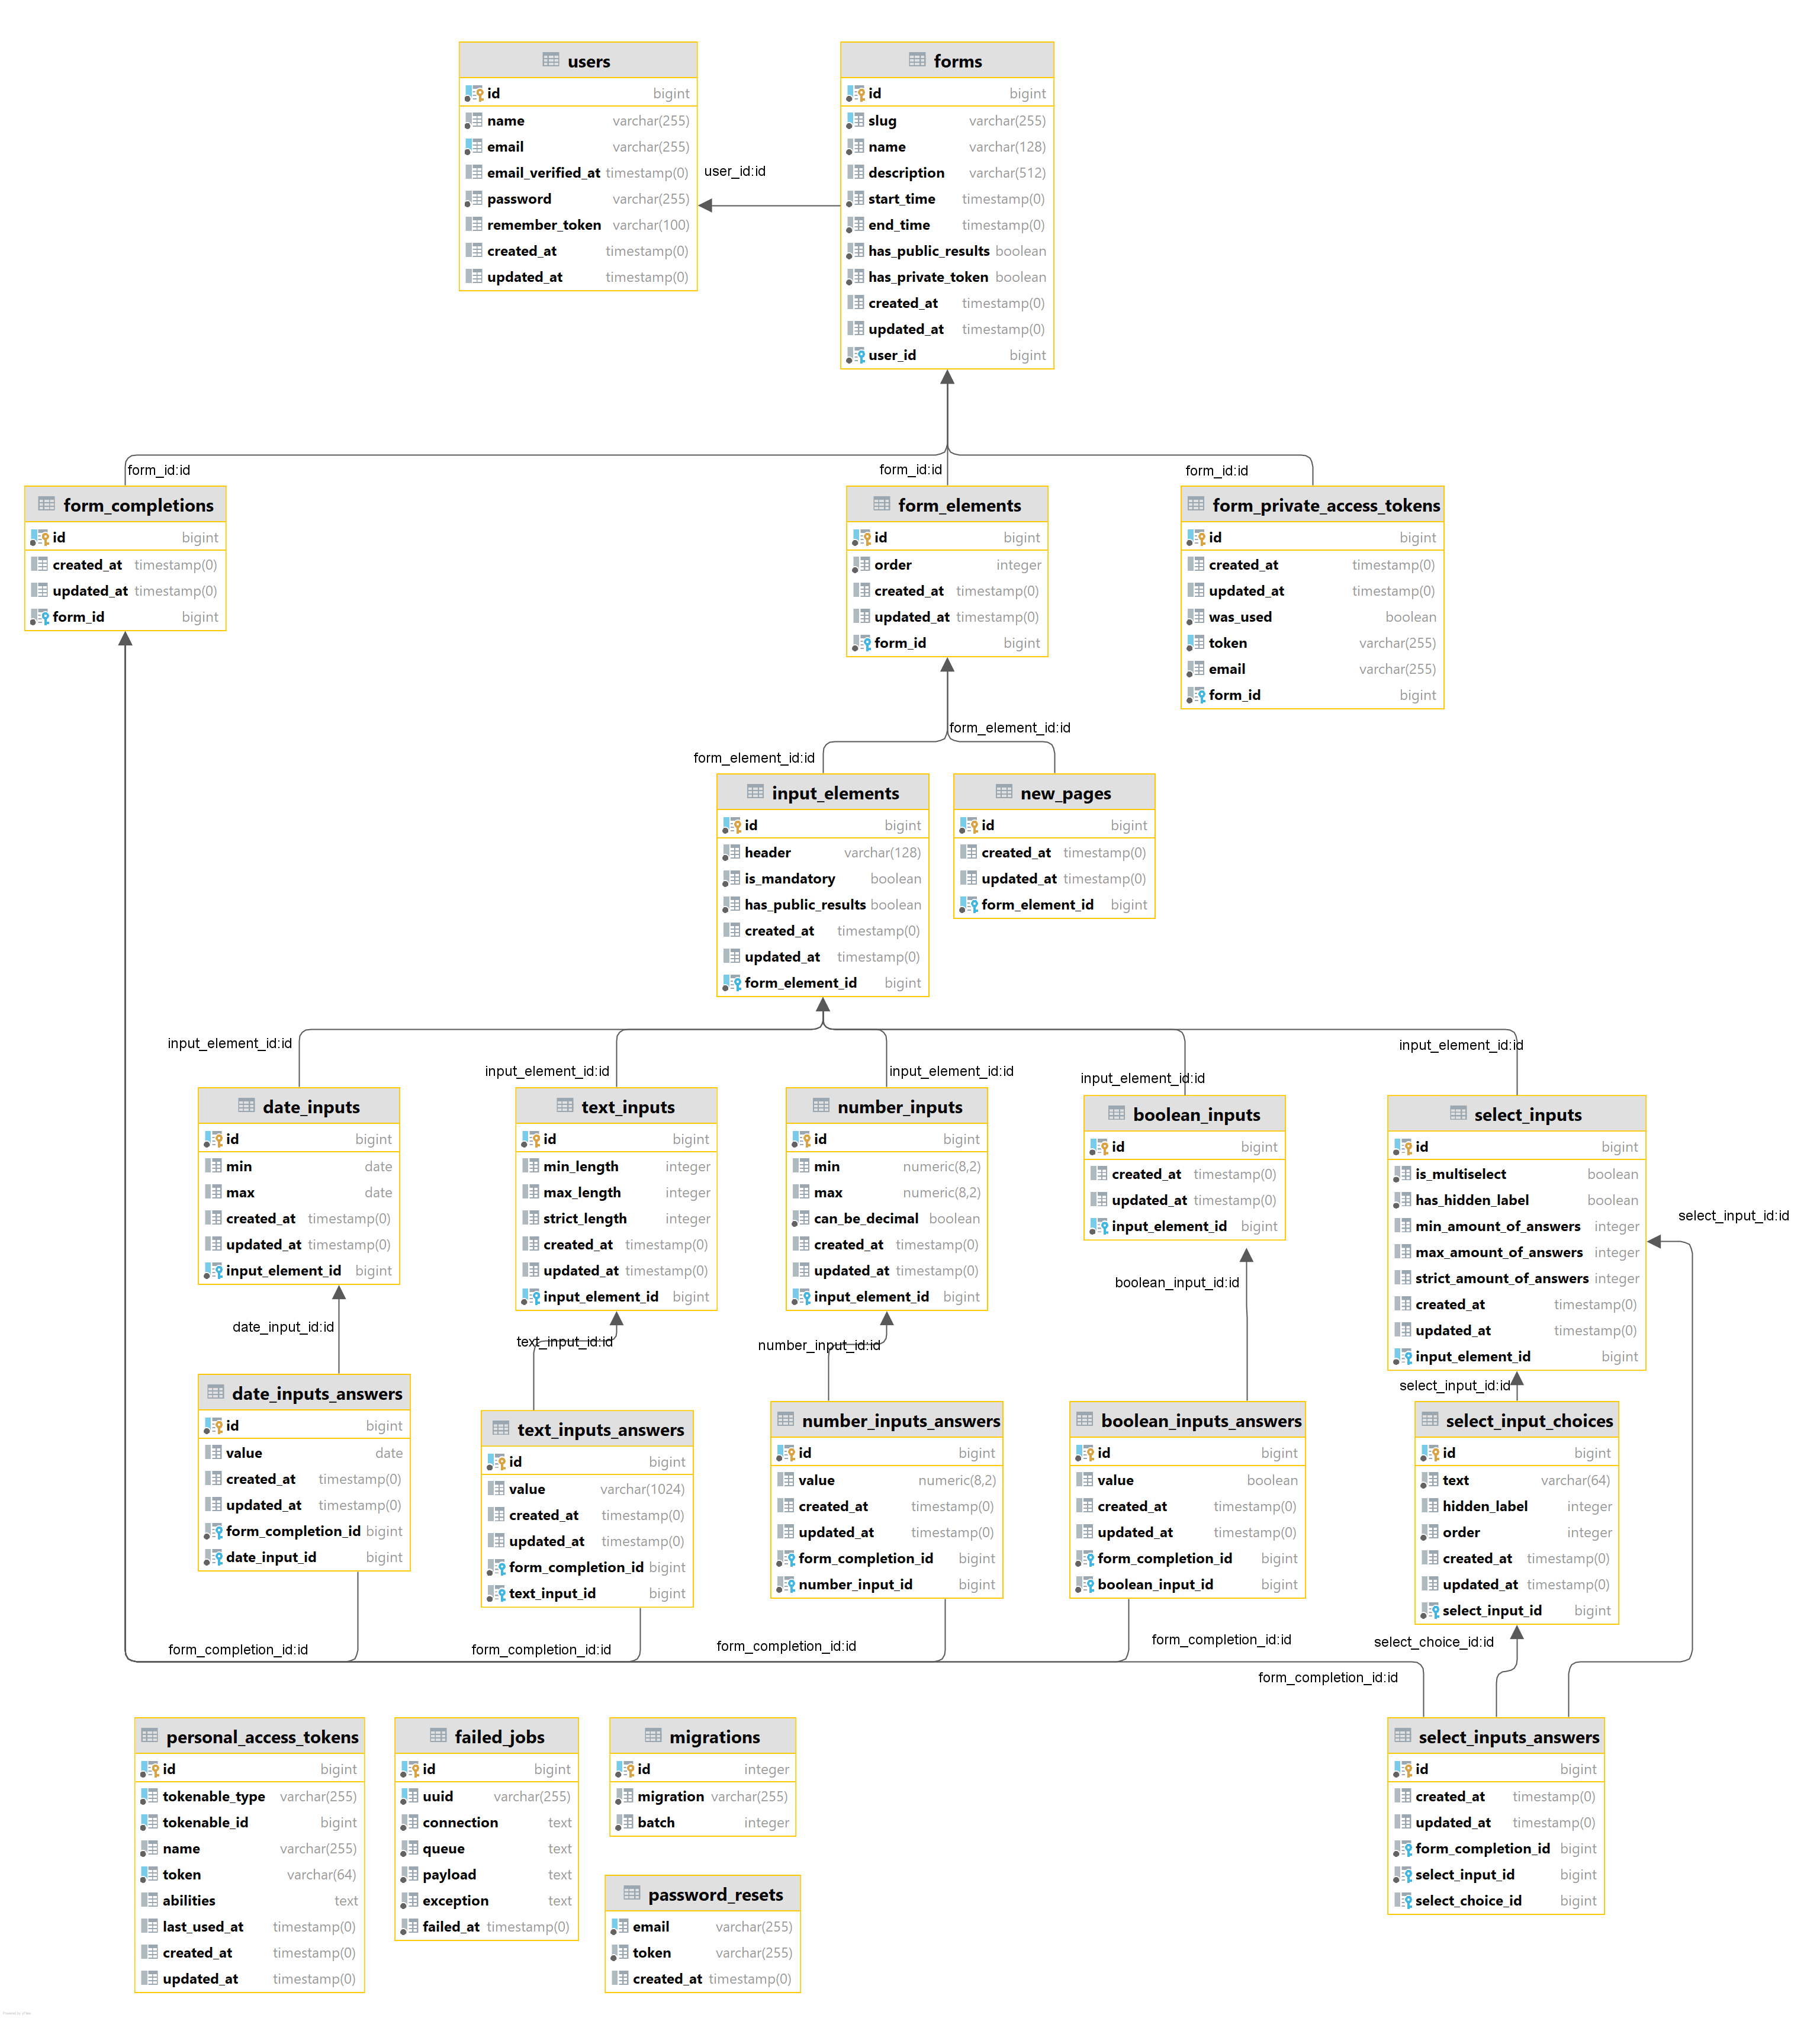
\includegraphics[height=0.61\paperheight]{img/appendix/db_diagram.png} %% vložení samotného obrátku
			\label{fig:db_diagram} %% označení až budeš chtít na obrázek odkazovat
		\end{figure}
	%pro školu
	%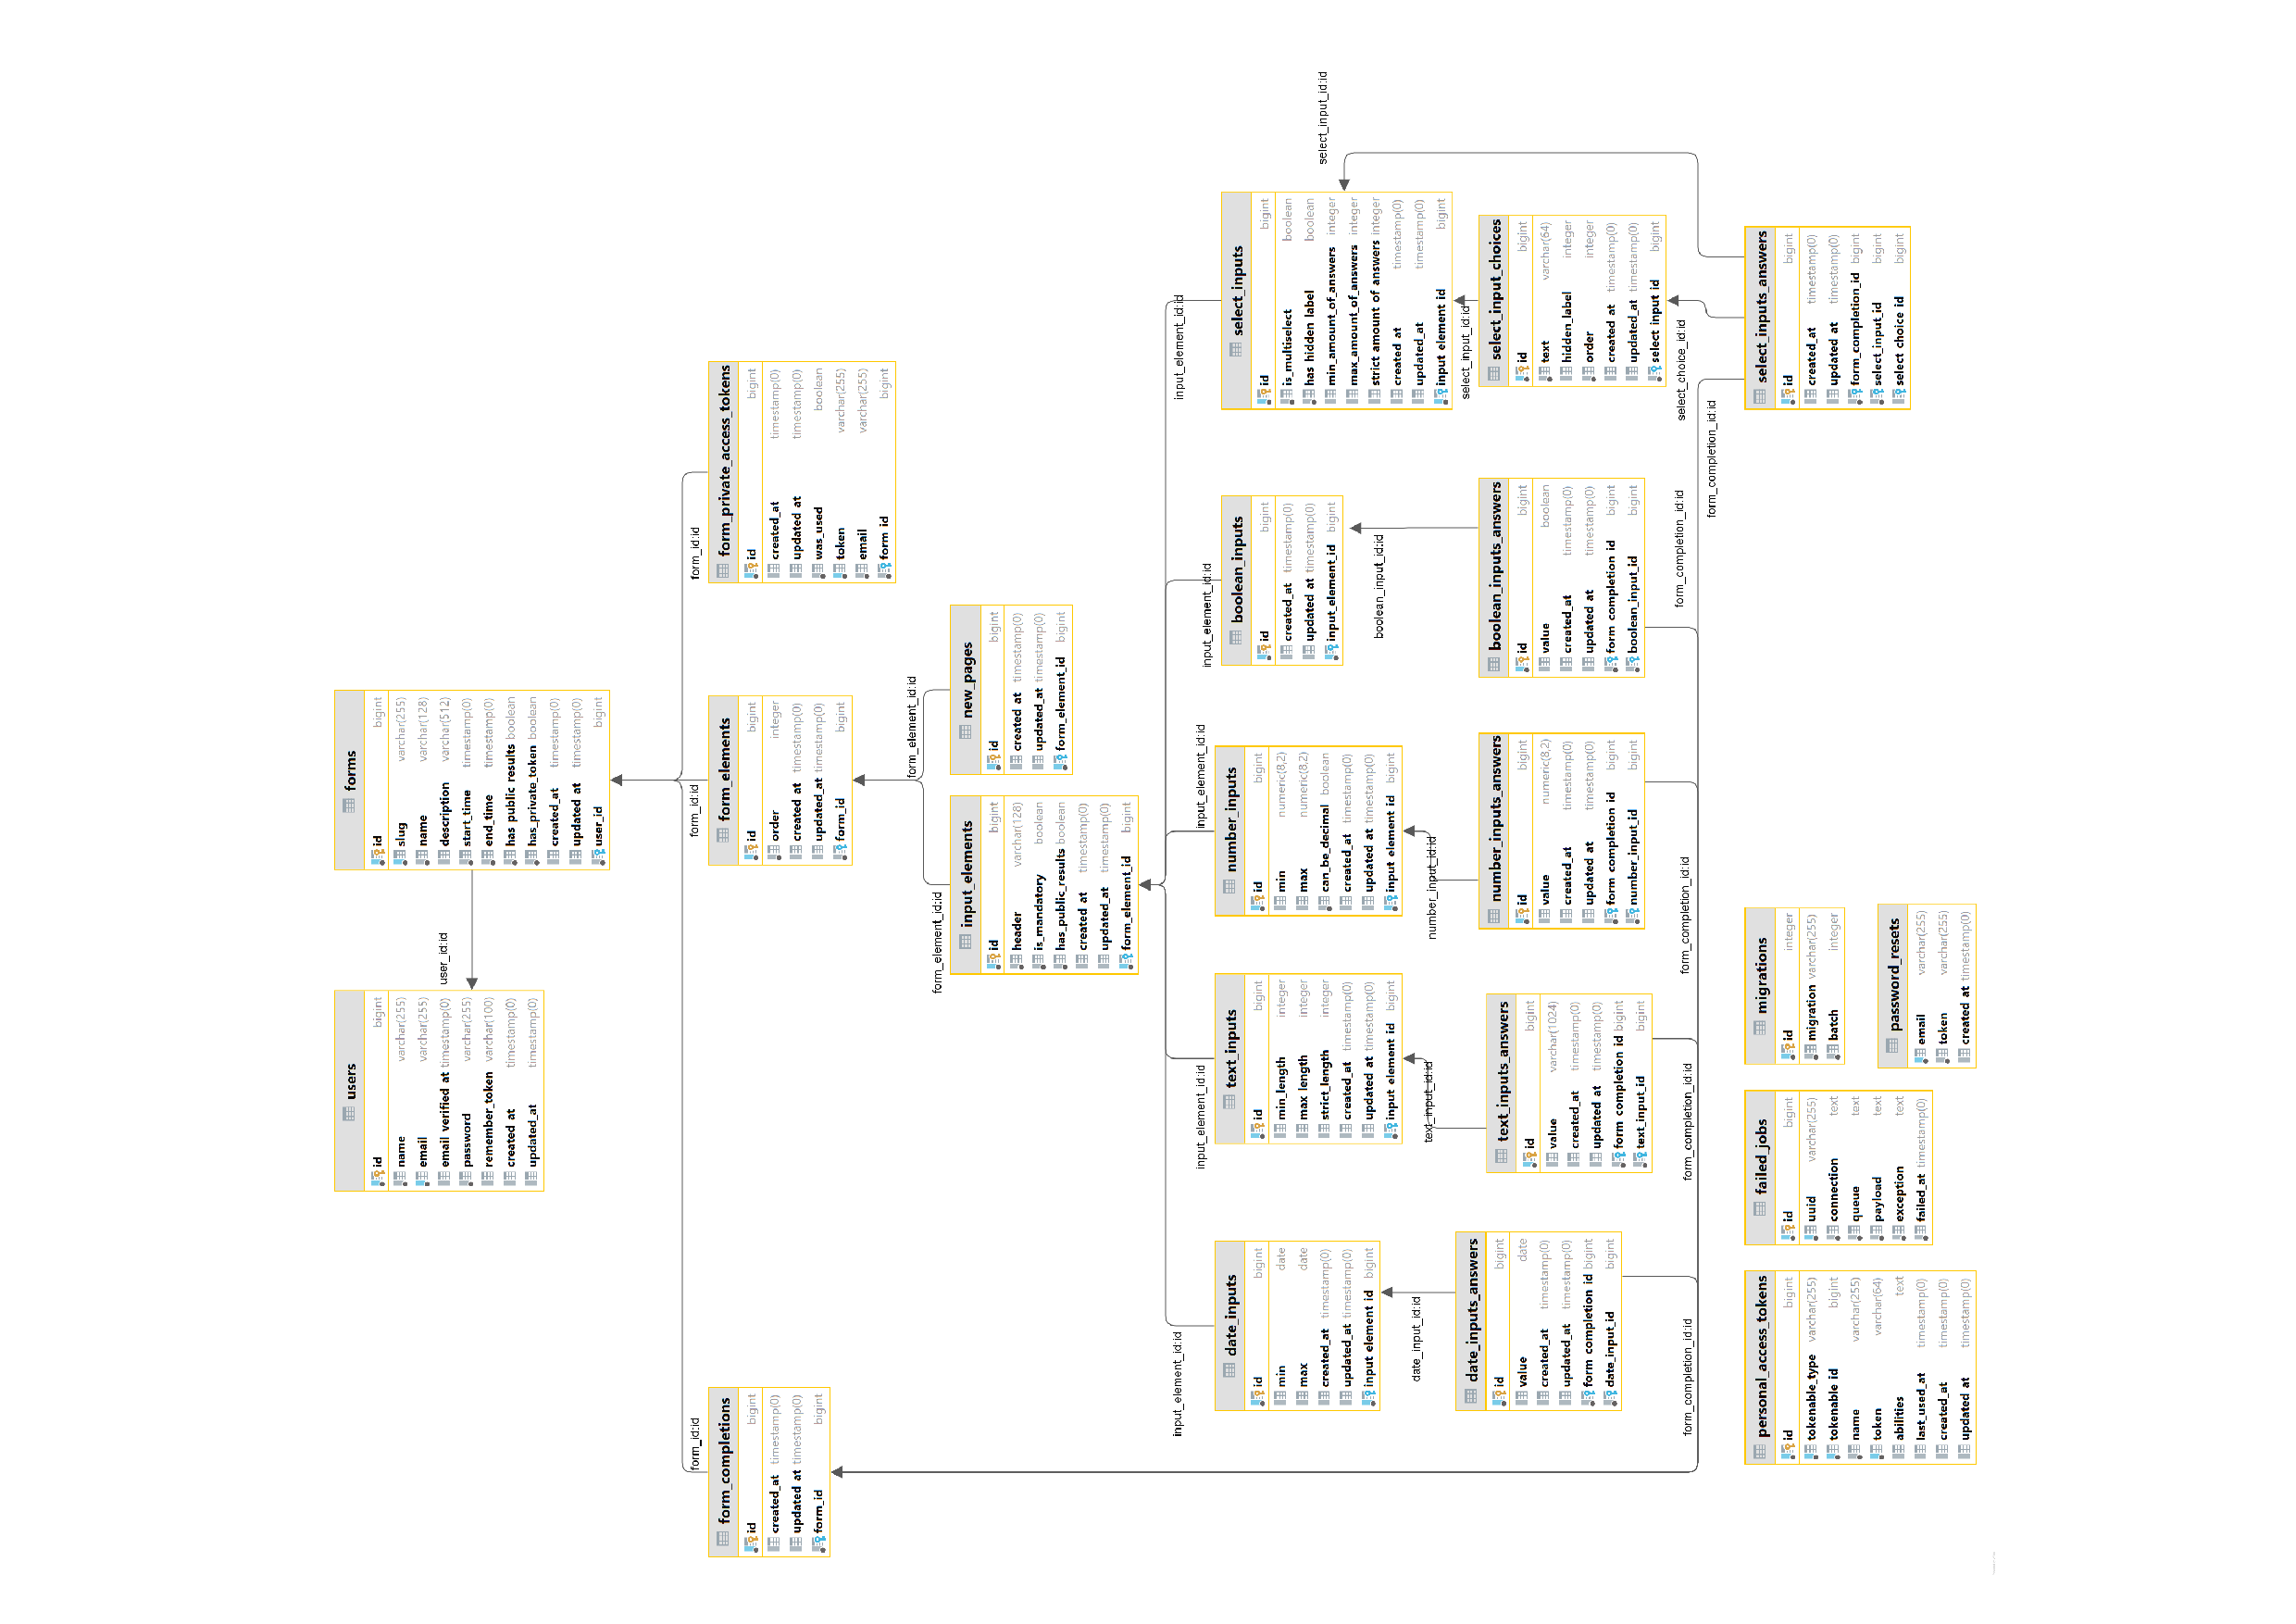
\includepdf[pages={1-},fitpaper]{pdf/db_diagram_A3.pdf}	
	%\cleardoublepage
	%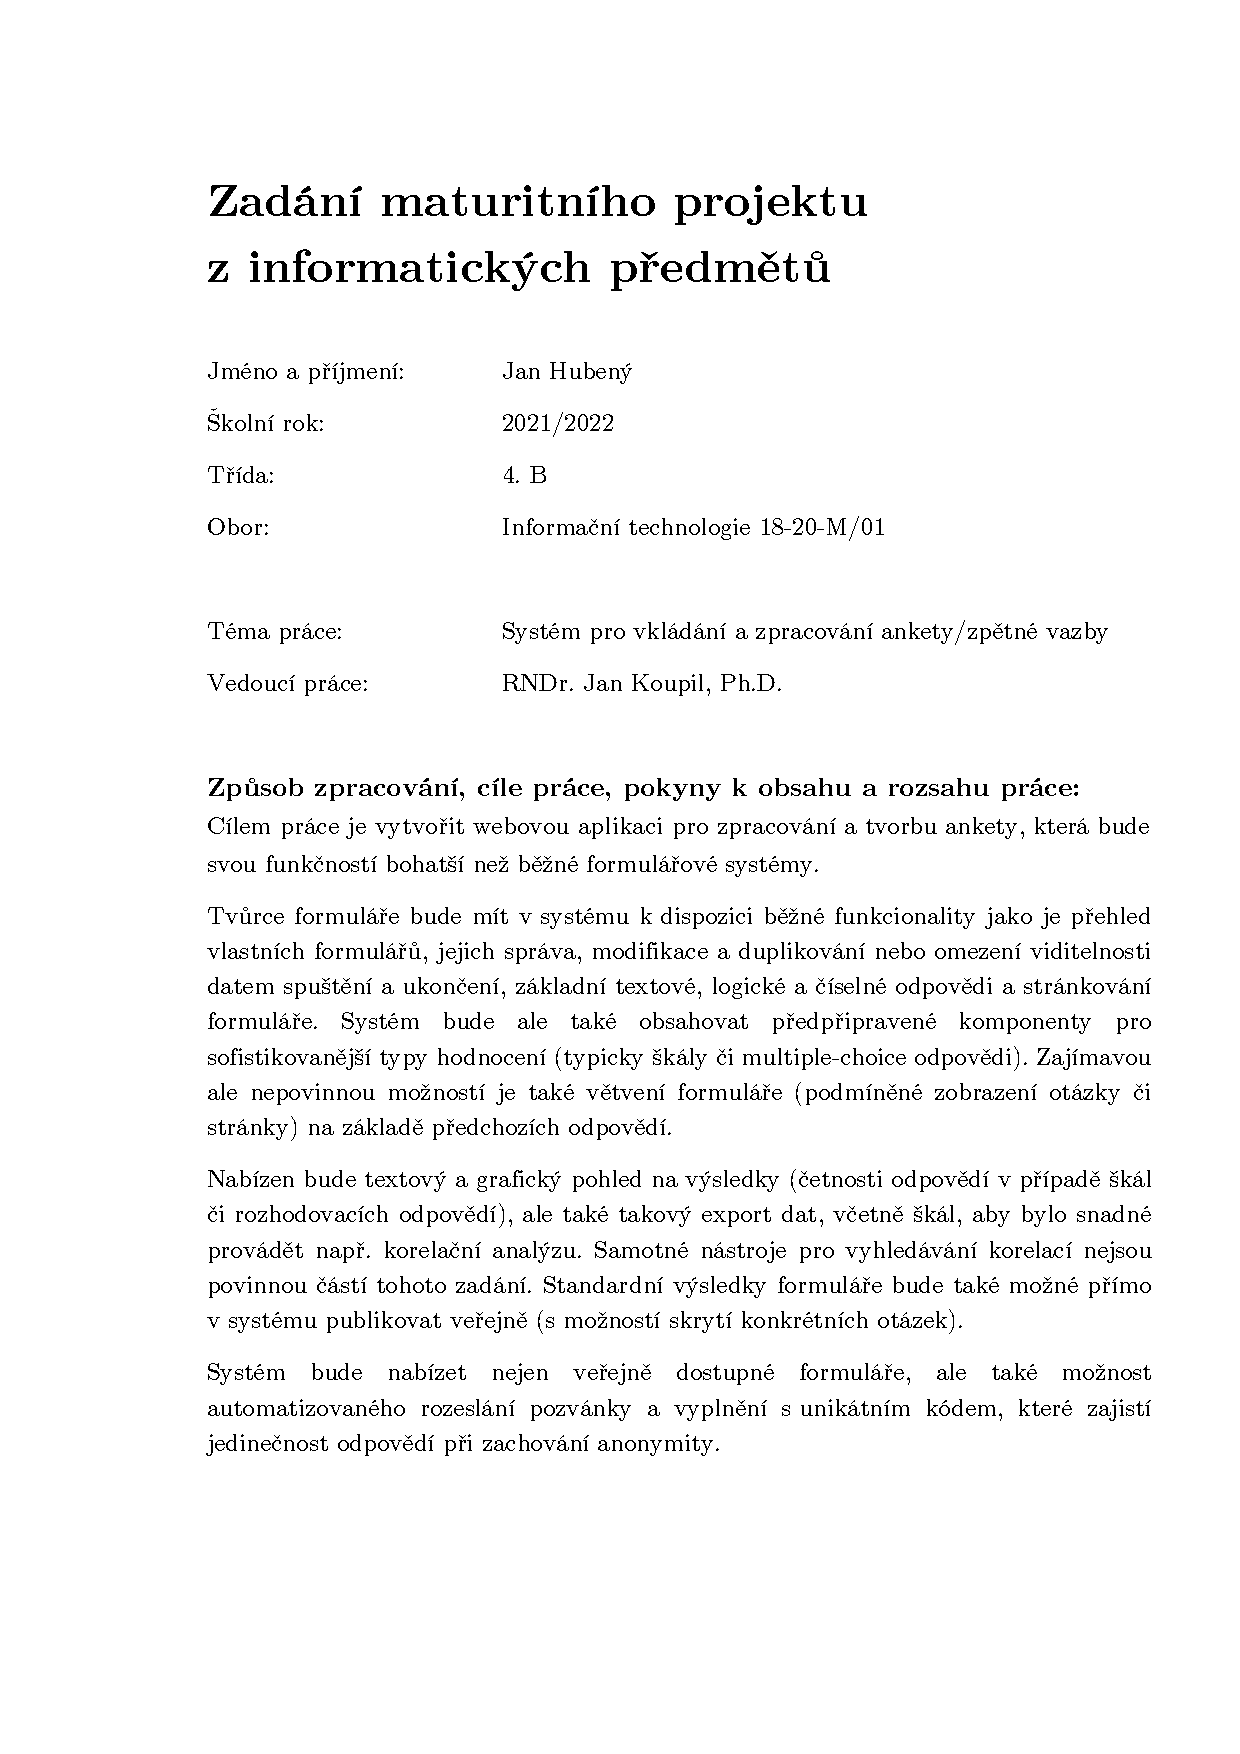
\includepdf[pages={1-}]{pdf/zadani.pdf}	

\end{document}